\documentclass[11pt]{beamer}
\usetheme{metropolis}
\usepackage[utf8]{inputenc}
\usepackage[english]{babel}
\usepackage[T1]{fontenc}
\usepackage{amsmath}
\usepackage{amsfonts}
\usepackage{amssymb}
\usepackage{bm}
\usepackage{subfig}
\usepackage{pgfplots}
\pgfplotsset{compat=newest}
\usepackage{multimedia}
%\usepackage{booktabs}
\newcommand{\Ex}{\mathbb{E}}
\newcommand{\Var}{\mathbb{V}\mathrm{ar}}
\newcommand{\Prob}{\mathbb{P}}
\DeclareMathOperator*{\argmin}{arg\,min}
\DeclareMathOperator*{\argmax}{arg\,max}
\newcommand{\Cov}{\textsf{Cov}}
\newcommand{\tra}{\mathrm{tr}}
\newcommand{\yobs}{\bm{y}^{\mathrm{obs}}}
\newcommand{\kest}{\hat{\bm{k}}}
\newcommand{\Uspace}{\mathbb{U}}
\newcommand{\Kspace}{\mathbb{K}}
\usepackage[duration=25, lastminutes=5]{pdfpcnotes}
\usetikzlibrary{positioning}
\DeclareMathOperator*{\KL}{\textsf{KL}}
\graphicspath{{../Figures/}}

\definecolor{blkcol}{HTML}{E1E1EA}
\definecolor{blkcol2}{RGB}{209, 224, 224}

% \definecolor{BlueTOL}{HTML}{222255}
% \definecolor{BrownTOL}{HTML}{666633}
% \definecolor{GreenTOL}{HTML}{225522}
% \setbeamercolor{normal text}{fg=BlueTOL,bg=white}
% \setbeamercolor{alerted text}{fg=BrownTOL}
% \setbeamercolor{example text}{fg=GreenTOL}

\setbeamercolor{block title}{bg = blkcol}
\setbeamercolor{block body}{bg = blkcol!50}

\setbeamerfont{author}{size=\footnotesize}

\title{Parameter control in the presence of uncertainties}
\subtitle{Robust Estimation of Bottom friction}
\author{{\large \bf Victor Trappler} \hfill \texttt{victor.trappler@univ-grenoble-alpes.fr} \\
  É. Arnaud, L. Debreu, A. Vidard \\
  AIRSEA Research team (Inria)\hfill \texttt{team.inria.fr/airsea/en/}\\
  Laboratoire Jean Kuntzmann}


\institute{\begin{center}

\includegraphics[scale=0.20]{INRIA_SCIENTIFIQUE_UK_CMJN}

\includegraphics[scale=0.20]{ljk}
\end{center}}

\date{\textbf{GdR MASCOTNUM, Grenoble, 2020}
  % {\bf } \today
}
\setcounter{tocdepth}{1}

\begin{document}
\frame{
   \pnote{Hello everyone, my name is Victor Trappler, I'm a PhD student in the AIRSEA team in Grenoble, under the supervision of Élise Arnaud, Arthur Vidard and Laurent Debreu.


I'm here to present some of the work entitled ``Parameter Control in the Presence of uncertainties''
}
  \maketitle
\metroset{sectionpage=none, subsectionpage=none}
}
\section{Introduction}

\frame{
  \frametitle{Processus of modelling of physical systems}
 %  \begin{center}
%   \scalebox{1}{\input{../Figures/flowchart_modelling_uncertainties_vert}}
% \end{center}  
  Uncertainties and errors are introduced at each stage of the modelling, by simplifications, parametrizations\dots

  In the end, we have a set of parameters we want to calibrate, but how can we be sure that this calibration is acting upon the errors of the modelling, and does not compensate the effect of the natural variability of the physical system?
  \pnote{During the whole process of the modelling of a physical system, that is from the observation of a natural phenomenon, to the simulation using numerical methods, we introduce uncertainties.    
    Those uncertainties take the form of errors introduced by the simplifications, discretizations and parametrizations needed to represent things numerically.

    In the end, we have a set of parameters, that we need to calibrate, but during this phase of calibration, how can we be sure that we try to correct only the error due to the parametrization, and are not compensating errors coming from others sources.}
}
\frame{
\frametitle{Outline}
\tableofcontents
\pnote{We are first going to see what problems arise when considering the deterministic case. This will lead us to introduce uncertainties, and then how to define robustness. Finally, we are going to see quickly how surrogate models can help us tackle these issues, especially those linked to the curse of dimensionality}
}
\metroset{sectionpage=progressbar, subsectionpage=none}

\section{Deterministic problem}
\frame[t]{
\frametitle{Computer code and inverse problem}
\begin{itemize}
	\item[Input] 
	\begin{itemize}
		\item $\bm{k}$: Control parameter%Bottom friction (spatially distributed)
		\item $\bm{u}$: Environmental variables (fixed and known)
	\end{itemize}
	\item[Output] \begin{itemize}
          \item $\mathcal{M}(\bm{k},\bm{u})$: Quantity to be compared to observations%Sea surface height, at predetermined time of the simulation and at certain location
	\end{itemize}
      \end{itemize}
      \vfill
\only<1>{\tikzstyle{block} = [rectangle, draw, fill=blue!20, 
     text centered, minimum width=1cm]

\tikzstyle{block2} = [rectangle, draw, fill=green!20, 
     text centered, rounded corners, minimum width=1cm]

\tikzstyle{LHS}=[rectangle, draw, text centered]

\begin{tikzpicture}[node distance=3cm]

\node [align = center] at (0,0) (input) {Control variable \\$K \in \mathcal{K}$};
%\node [align = center] at (4,1.5) (envir) {Environmental variables \\$\bm{u} \in \mathcal{U}$ fixed};
\node [align = center] at (4,1.5) (envir) {Environmental variables \\$\bm{x}_e \in \mathbb{X}$ fixed};

\node[block] at (4,0)(code){Direct Simulation};

\node[align = center] at (8,0) (output) {$W(K)$}; %\\ $\Rightarrow j(K)$};

\draw[->] (input) -- (code);
\draw[->] (envir) -- (code);
\draw[->] (code) -- (output);

\end{tikzpicture}}
\only<2>{\usetikzlibrary{positioning}
% \tikzstyle{block} = [rectangle, draw, fill=blue!30, 
%     text centered, minimum width=3em] 
 \tikzstyle{block} = [rectangle, draw, fill=blkcol, 
      text centered, minimum width=3em]

\tikzstyle{block2} = [rectangle, draw, fill=blkcol2, 
     text centered, rounded corners, minimum width=3em]

% \tikzstyle{block2} = [rectangle, draw, fill=blkcol2, 
%      text centered, rounded corners, minimum width=3em]

\tikzstyle{LHS}=[rectangle, draw, text centered]

\begin{tikzpicture}

%\node [align = center] at (0,0) (input) {Control variable \\$\mathbf{k} \in \mathbb{K}$};
\node [align = center] at (0,0) (input) {Control variable \\$\bm{k} \in \mathbb{K}$};
\node[block] at (4,0) (code){Direct Simulation};
%\node [align = center, above =of  code ] (envir) {Environmental variables \\$\mathbf{u} \in \mathbb{U}$ fixed};
\node [align = center] at (4,1.5) (envir) {Environmental variables \\$\bm{u} \in \mathbb{U}$ fixed};




%\node[align = center, right =of  code] (output) {$M(\mathbf{k})$};
\node[align = center] at (8,0) (output) {$\mathcal{M}(\bm{k},\bm{u})$};
%\node [align = center, right =of  inv, below = of output]  (obs) {$\mathbf{y}$};
\node [align = center] at (8,-1) (obs) {$\yobs$};
\node[block] at (4,-1) (inv) {Inverse Problem};

\draw[->] (input) -- (code);
\draw[->] (envir) -- (code);
\draw[->] (code) -- (output);

 % \node [align = center] at (0,0) (input) {$Y = \mathbb{H}M(K_{\mathrm{ref}})$};
 % \node [align = center] at (4,1.5) (envir) {Environmental variables \\$X_e$ r.v.};

 % \node[block] at (4,0)(code){"Inverse Problem"};

% \node[align = center] at (8,0) (output) {$K$};

\draw[->] (input) -- (code);
% \draw[->] (envir) -- (code);
\draw[->] (code) -- (output);
\draw[->] (output) -- (obs) ;
\draw[->] (inv) -|(input) ;
\draw[->] (obs) -- (inv);
\end{tikzpicture}}

\pnote{In quite a classical setting, we assume that we have a model M, that takes two inputs: k the control variable, that we aim at calibrating, and u some environmental variables, that we consider fixed and knowns.


Now, to have an inverse problem, we have some observations, that are kinda linked to the model, and from those observations we wish to get back the parameter k from the start.
}
}
\frame{
\frametitle{Data assimilation framework}
We have $\yobs = \mathcal{M}(\bm{k}_{\mathrm{obs}},\bm{u}_{\mathrm{obs}})$ with $\bm{u}_{\mathrm{obs}} = \bm{u}$
\begin{equation*}
\hat{\bm{k}} = \argmin_{\bm{k}\in\Kspace} J(\bm{k}) = \argmin_{\bm{k}\in\Kspace}\frac12 \|\mathcal{M}(\bm{k},\bm{u}) - \bm{y}^{\mathrm{obs}} \|^2
\end{equation*}
\begin{itemize}
\item[$\rightarrow$] Deterministic optimization problem
\item[$\rightarrow$] Possibly add regularization
\item[$\rightarrow$] Classical methods: Adjoint gradient and Gradient-descent
\end{itemize}
BUT
\begin{itemize}
\item What if $\bm{u} \neq \bm{u}_{\mathrm{obs}}$?
\item Does $\hat{\bm{k}}$ compensate the errors brought by this misspecification?
% \item How well will $\bm{\hat{k}}$ perform under other conditions?
\end{itemize}
\pnote{
  In practice: we assume that the observations have been generated in a twin experiment framework, using the model and two references values kobs and uobs, uobs that is known. Using the least square approach, we define J, a cost function, as the sum of the squares of the difference.


  This is a deterministic optimisation problem, that we can solve using classical methods such as adjoint gradient. Notice that the u used in the optimisation procedure is known.

  But what if it is not, to say that there is a difference between uobs and u. The minimisation procedure is supposed to correct the error of k but how about the error due to uobs and u used in the minimisation ?}
}
\frame{
\frametitle{Context}
\begin{itemize}
\item The friction $\bm{k}$ of the ocean bed has an influence on the water circulation
\item Depends on the type and/or characteristic length of the asperities 
\item Subgrid phenomenon
\item $\bm{u}$ parametrizes the BC
\end{itemize}
\begin{center}
\scalebox{.9}{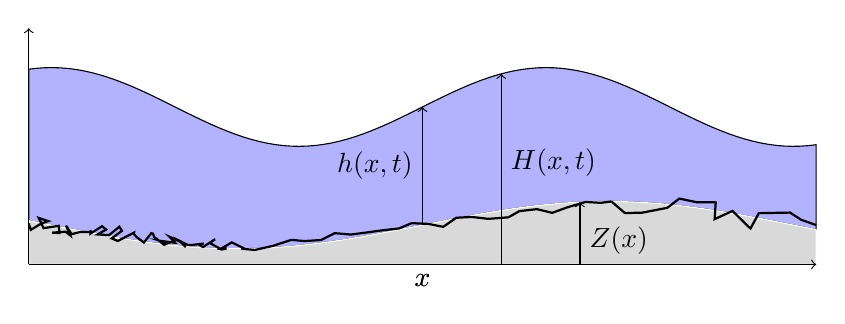
\begin{tikzpicture}
\usetikzlibrary{decorations.pathmorphing}

\definecolor{copper}{rgb}{0.69, 0.25, 0.21}
\definecolor{tin}{rgb}{0.7, 0.7, 0.7}

\tikzset{
  rugous1/.style = {black, thick,
    decoration={random steps,segment length=0.05cm,amplitude=.1cm}
  },
}
\tikzset{
  rugous2/.style = {black, thick,
    decoration={random steps,segment length=0.2cm,amplitude=.05cm}
  },
}
\tikzset{
  rugous3/.style = {black, thick,
    decoration={random steps,segment length=0.2cm,amplitude=.15cm}
  },
}

\filldraw [fill = blue!30]
   plot [samples = 100,domain = -5:5] (\x, {0.5*sin(\x r) + 2} )
-- plot [samples = 100,domain = 5:-5] (\x, {0.3*sin(\x/1.5 r)+0.5})
-- cycle;

\filldraw[fill = gray!30, draw = white]
   plot [samples = 100,domain = -5:5] (\x, {0.3*sin(\x/1.5 r)+0.5})
-- plot [samples = 100,domain = 5:-5] (\x, 0)
-- cycle;

\draw[rugous1, decorate](-5,0.52) -- (-2.3,0.2);
\draw[rugous2, decorate](-2.3,0.2) -- (2.4,0.8);
\draw[rugous3, decorate](2.4,0.8) -- (5,0.5);

\draw[->] (-5,0) -- (5,0);
\draw (0,0) node[below] {$x$};



\draw[->] (-5,0) -- (-5,3);

\draw[->] (0,0.5) -- (0,2);
\draw (0, 1.25) node[left] {$h(x,t)$} ;
\draw (0,0) node[below] {$x$};
\draw[->] (2,0) -- (2,{0.3*sin(2/1.5 r)+0.5});
\draw (2, 0.3) node[right] {$Z(x)$} ;
\draw[->] (1,0) -- (1,{0.5*sin(1 r)+2});
\draw (1, 1.3) node[right] {$H(x,t)$} ;
\end{tikzpicture}}
\end{center}
\pnote{
  The problem here at stakes is the estimation of the bottom friction.

  The bottom friction k has an influence on the oceanic circulation, as it dissipates some energy by turbulences.
  This friction parameter depends on the type of sediments, and more particularly, on the characteristic length of the asperities. Something that is hard to observe directly.
  In oceans modelling, this is a subgrid phenomenon.

  The environmental variable u parametrizes the BC, for instance the relative amplitude of tidal components.
  }
}


\section{Dealing with uncertainties}
\frame{
  \frametitle{Different types of uncertainties}
  \begin{block}{Epistemic or aleatoric uncertainties?~\cite{walker_defining_2003}}
\begin{itemize}
\item Epistemic uncertainties: From a lack of knowledge, that can be reduced with more research/exploration
\item Aleatoric uncertainties: From the inherent variability of the system studied, operating conditions
\end{itemize}
\end{block}
$\rightarrow$ But where to draw the line?

Our goal is to take into account the aleatoric uncertainties in the estimation of our parameter.
\pnote{
  We said earlier that there are a lot of uncertainties everywhere basically. But we can make a rough distinction between two types:

  - First, the epistemic uncertainties that result from a lack of knowledge, but can be reduce. An example is the uncertainty during the estimation of the mean value. The more samples you take, the less uncertainty there is on your estimation

  - Secondly, there is the aleatoric uncertainty, that comes from the inherent variability of the system studied. Think of the different values that a random variable takes.

  Our goal, is then to be able to reduce the epistemic uncertainty on the value of k to use, while taking into account the aleatoric uncertainty.
}
}

\frame[t]{
\frametitle{Aleatoric uncertainties}
Instead of considering $\bm{u}$ fixed, we consider that $\bm{U}$ is a random variable (pdf $\pi(\bm{u})$), and the output of the model depends on its realization. \\
\vfill
\only<1>{\usetikzlibrary{positioning}
% \tikzstyle{block} = [rectangle, draw, fill=blue!30, 
%     text centered, minimum width=3em] 
 \tikzstyle{block} = [rectangle, draw, fill=blkcol, 
      text centered, minimum width=3em]

\tikzstyle{block2} = [rectangle, draw, fill=blkcol2, 
     text centered, rounded corners, minimum width=3em]

% \tikzstyle{block2} = [rectangle, draw, fill=blkcol2, 
%      text centered, rounded corners, minimum width=3em]

\tikzstyle{LHS}=[rectangle, draw, text centered]

\begin{tikzpicture}

%\node [align = center] at (0,0) (input) {Control variable \\$\mathbf{k} \in \mathbb{K}$};
\node [align = center] at (0,0) (input) {Control variable \\$\bm{k} \in \mathbb{K}$};
\node[block] at (4,0) (code){Direct Simulation};
%\node [align = center, above =of  code ] (envir) {Environmental variables \\$\mathbf{u} \in \mathbb{U}$ fixed};
\node [align = center] at (4,1.5) (envir) {Environmental variables \\$\bm{u} \in \mathbb{U}$ fixed};




%\node[align = center, right =of  code] (output) {$M(\mathbf{k})$};
\node[align = center] at (8,0) (output) {$\mathcal{M}(\bm{k},\bm{u})$};
%\node [align = center, right =of  inv, below = of output]  (obs) {$\mathbf{y}$};
\node [align = center] at (8,-1) (obs) {$\yobs$};
\node[block] at (4,-1) (inv) {Inverse Problem};

\draw[->] (input) -- (code);
\draw[->] (envir) -- (code);
\draw[->] (code) -- (output);

 % \node [align = center] at (0,0) (input) {$Y = \mathbb{H}M(K_{\mathrm{ref}})$};
 % \node [align = center] at (4,1.5) (envir) {Environmental variables \\$X_e$ r.v.};

 % \node[block] at (4,0)(code){"Inverse Problem"};

% \node[align = center] at (8,0) (output) {$K$};

\draw[->] (input) -- (code);
% \draw[->] (envir) -- (code);
\draw[->] (code) -- (output);
\draw[->] (output) -- (obs) ;
\draw[->] (inv) -|(input) ;
\draw[->] (obs) -- (inv);
\end{tikzpicture}}
\only<2>{
\tikzstyle{block} = [rectangle, draw, fill=blkcol, 
     text centered, minimum width=1cm]
\tikzstyle{block2} = [rectangle, draw, fill=blkcol2, 
     text centered, rounded corners, minimum width=1cm]

\tikzstyle{LHS}=[rectangle, draw, text centered]

\begin{tikzpicture}[node distance=3cm]

\node [align = center] at (0,0) (input) {Control variable \\$\bm{k} \in \mathcal{K}$};
\node [align = center] at (4,1.5) (envir) {Environmental variables \\\alert<2>{$\bm{U}$ random}};
\node[block] at (4,0)(code){Direct Simulation};
\node[align = center] at (8,0) (output) {$W(\alert<2>{\bm{U}},\bm{k})$};
\node [align = center] at (8,-1) (obs) {$\yobs$};
\node[block] at (4,-1) (inv) {Inverse Problem};
\draw[->] (input) -- (code);
\draw[->] (envir) -- (code);
\draw[->] (code) -- (output);
\draw[->] (inv) -|(input) ;
\draw[->] (obs) -- (inv);
\draw[->] (output) -- (obs);
\end{tikzpicture}}
\vfill


\pnote{
  As hinted before, we are going to model the aleatoric uncertainty on u by a random variable.
  The inverse problem considered before becomes now the following, and the output of the model becomes a random variable
 }
}

\frame{
\frametitle{The cost function as a random variable}
\begin{itemize}
\item Output of the computer code ($\bm{u}$ is an input):
\begin{equation*}
    \mathcal{M}(\bm{k},\alert{\bm{u}})
\end{equation*}
\item The (deterministic) quadratic error is now
\begin{equation*}   
  J(\bm{k},\alert{\bm{u}}) =  \frac12\|\mathcal{M}(\bm{k},\alert{\bm{u}}) - \yobs\|^2
\end{equation*}
\end{itemize}

\begin{equation*}
  ''\hat{\bm{k}} = \argmin_{\bm{k}\in\Kspace} J(\bm{k},\alert{\bm{u}})'' \text{ but what can we do about } \bm{u} ?
\end{equation*}
\pnote{
  In our study, the models are deterministic, so we can control the inputs
  The cost function, becomes then a function of two inputs. We still wish to minimise with respect to k, but what can we do for u ? A first solution would be to set it to a fixed value, such as the mean of the random variable
  }
}

\frame{
  \frametitle{Toy Problem: Influence of misspecification of $\bm{u}_{\mathrm{obs}}$}
  Minimization performed on $\bm{k}\mapsto J\left(\bm{k},
    \Ex\left[\bm{U}\right]\right)$, for different $\bm{u}_{\mathrm{obs}}$: Naïve approach
  \begin{center}
    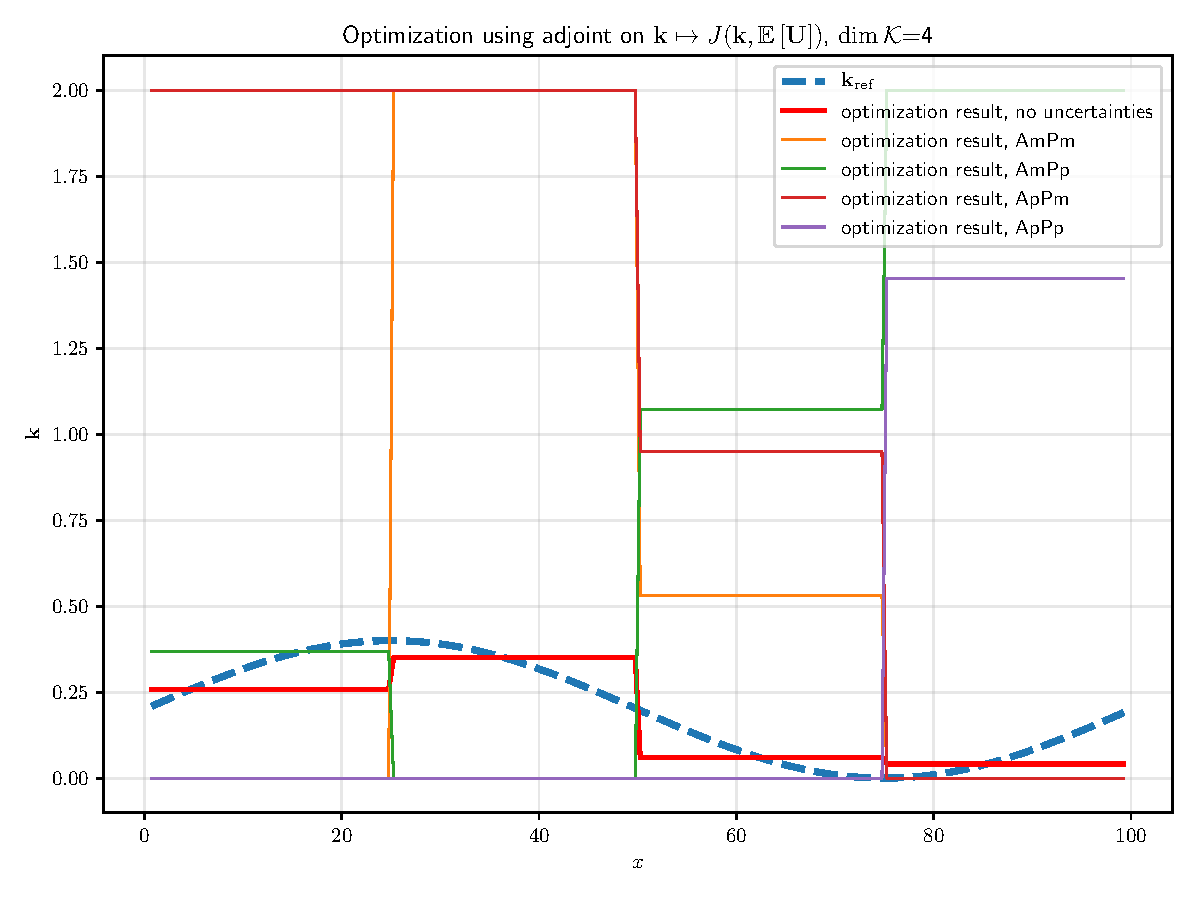
\includegraphics[width=.8\textwidth]{optimization_using_misspecified_uref_4d}
  \end{center}
  \pnote{
    To look first into this solution, we applied this to a toy problem based on the SWE.
    We set different observations using different uobs
    The real friction is the dashed sine curve at the bottom.
    When there is no difference, that is uobs equals the mean, the solution seems satisfying. But when there are differences, the estimations are not good at all. We can see that this solution is not really robust. Here finding a value k robust has to be understood as the ability for this k to perform reasonaly well under different operating conditions u. 
    }
}

\frame{
  \frametitle{Robust Estimation of parameters}
  \pnote{So basically, we have two main objectives:
    - First to find some criteria of robustness to estimate k
    - Be able to compute those estimates quickly
    This objectives requires some reflexion on first, being able to explore the U space quite efficiently, using design of experiments. Also, as k may be defined on every points of the mesh, we may want to be able to reduce the dimension of this to keep the computation tractable.
  }
  \begin{itemize}
    \item Main objectives:
    \begin{itemize}
    \item Define criteria of robustness, based on $J(\bm{k},\bm{u})$, that will depend on the final application
    \item For each criterion, be able to compute an estimate $\hat{\bm{k}}$ in a reasonable time
    \end{itemize}
  \item Questions to be answered along the way:
    \begin{itemize}
    \item Good exploration of $\Uspace$, based on the density of $\bm{U}$ (Design of Experiment: LHS, Monte-Carlo, OA,\dots~?)
    \item Deal with dimension of $\Kspace$?
    \end{itemize}
  \end{itemize}
}



\metroset{sectionpage=none, subsectionpage=progressbar}

\section{Robust minimization}

\subsection{Criteria of robustness}

\frame{
  \frametitle{Non-exhaustive list of ``Robust'' Objectives }
  \pnote{
    I'm going to present very quickly some estimates that can be considered robust, but will focus mainly on the last one.
    First we can think about minimising in the worst case sense. This usually leads to overly conservative estimates. We can also think about minimising the moments, such as the mean or the variance, or even combine them in a multiobjective setting by looking for the pareto front.

The main thing we've been working on is to see how can we get the best performance attainable, for each configuration u sampled
  }
\begin{itemize}
% \item Global Optimum: $ \min_{(\bm{k},\bm{u})} J(\bm{u},\bm{k})$ $ \longrightarrow $ EGO
\item Worst case~\cite{marzat_worst-case_2013}: $$ \min_{\bm{k} \in \Kspace} \left\{\max_{\bm{u} \in \Uspace} J(\bm{k},\bm{u})\right\}$$
\item M-robustness~\cite{lehman_designing_2004}: $$\min_{\bm{k}\in\Kspace} \Ex_{\bm{U}}\left[J(\bm{k},\bm{U})\right]$$
\item V-robustness~\cite{lehman_designing_2004}: $$\min_{\bm{k}\in\Kspace} \Var_{\bm{U}}\left[J(\bm{k},\bm{U})\right]$$
\item Multiobjective~\cite{baudoui_optimisation_2012}: $$ \text{Pareto frontier}
  $$
% \item Region of failure given by $J(\bm{k},\bm{u})>T$~\cite{bect_sequential_2012}: $$\max_{\bm{k} \in \Kspace} R(\bm{k}) = \max_{\bm{k}\in \Kspace} \Prob_{\bm{U}}\left[J(\bm{k},\bm{U}) \leq T \right]$$
\item Best performance attainable for each configuration $\bm{u} \sim \bm{U}$
\end{itemize}
}

% \frame{
%   \frametitle{Toy Problem: Minimization of mean value}
%   \vspace{-5ex}
%    \begin{center}
%     {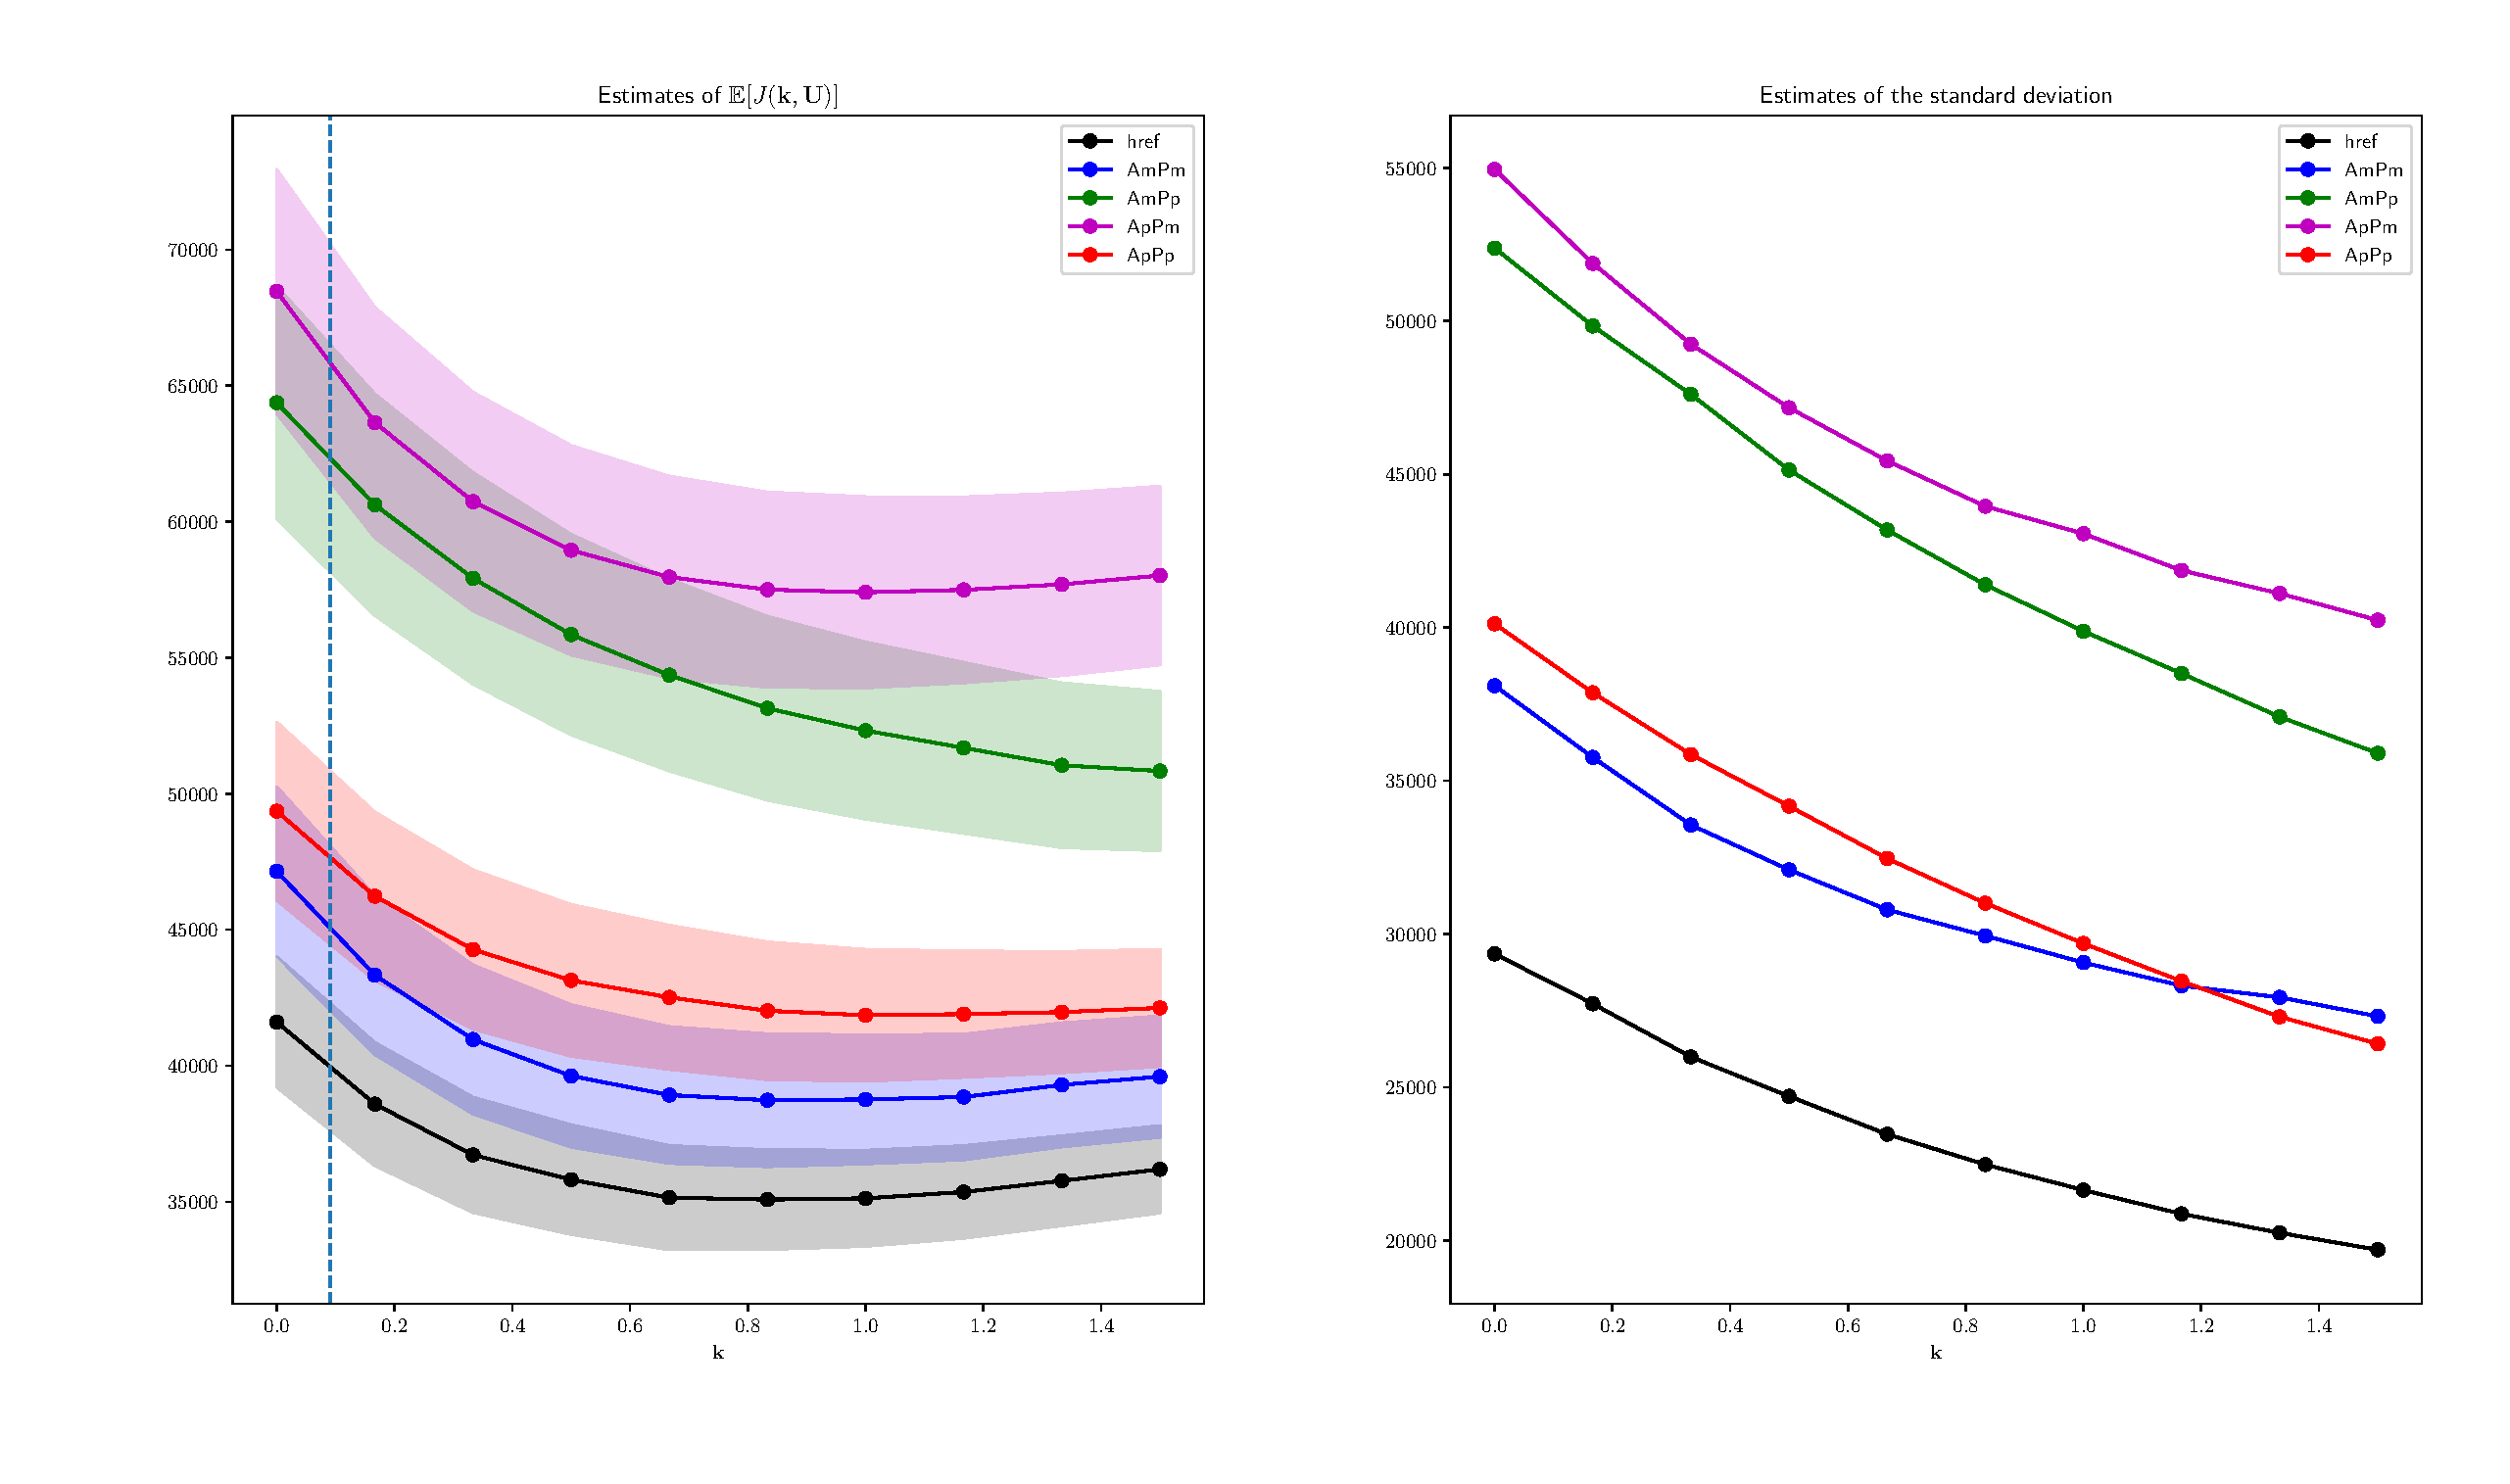
\includegraphics[height = .8\textheight, width = \linewidth]{mean_minimization_illustration}}
%   \end{center}
%   \vspace{-3ex}
%    $\longrightarrow$ Quite different from the value $\bm{k} \approx 0.1$ obtained by optimization knowing the true value of $\bm{u}_{\mathrm{ref}}$ 
% }

\frame{
  \frametitle{``Most Probable Estimate'', and relaxation}%

  \pnote{
    Basically, once a value u is sampled, the problem is deterministic, so under some assumption, we have a minimiser kstar that is a function of u


    Keeping in mind the random nature of U, we can define the random variable Kstar, and its density (if it is defined), can be seen as the frequency of which a value k is optimal.


    That is an interesting information, but we can have a little more than that. We may want to include k that yield values of the cost function close to a minimum. To do that, we introduce a relaxation of the equality constraint with alpha, so that for a given u, we consider acceptable the k that give values of the cost function between Jstar, the optimal value and alpha times Jstar
    So finally, we compute the probability that this given k is acceptable with respect to the level alpha
    }
  Main idea: For each $\bm{u} \sim \bm{U}$, compare the value of the cost function to its optimal value $J^*(\bm{u})$ and define
  $\bm{k}^*(\bm{u}) = \argmin_{\bm{k}\in\Kspace} J(\bm{k},\bm{u})$
  \pause
    % \begin{columns}
    %   \begin{column}{0.6\textwidth}
      The minimizer as a random variable:
      \begin{equation*}
        \bm{K}^* = \argmin_{\bm{k}\in\Kspace} J(\bm{k},\alert<1>{\bm{U}})
      \end{equation*}
      $\longrightarrow$ estimate its density (how often is the value $\bm{k}$ a minimizer)
      \begin{align*}
        p_{\bm{K}^*}(\bm{k})%\,\mathrm{d} \bm{k} & = \Prob\left[\bm{K}^* \in \left[\bm{k},\bm{k}+\mathrm{d}\bm{k} \right]\right] \\
                                        %        & =\Prob\left[\argmin J(\bm{k}, \bm{U}) \in \left[\bm{k},\bm{k}+\mathrm{d}\bm{k} \right]\right] \\
                                               &= "\Prob\left[J(\bm{k},\bm{U})= J^*(\bm{U}) \right]"                                               % & \Prob\left[ J(\bm{U}) \leq J(\bm{k}, \bm{U}) \forall \bm{k} \in \left[\bm{k},\bm{k}+\mathrm{d}\bm{k} \right]\right]
      \end{align*}
      \pause
      How to take into account values not optimal, but not too far either
      $\longrightarrow$ relaxation of the equality with $\alpha> 1$:
      \begin{equation*}
        \Gamma_{\alpha}(\bm{k}) = \Prob_{\bm{U}}\left[J(\bm{k},\bm{U}) \leq \alpha J^*(\bm{U}) \right]
      \end{equation*}
      % \begin{align*}
      %   R(\bm{k}) & = \Prob_{\bm{U}}\left[\bm{k} = \argmin_{\tilde{\bm{k}}} J(\tilde{\bm{k}},\bm{U}) \right] \\
      %   \only<1>{\phantom{R_{\alpha}(\bm{k})} & = \Prob_{\bm{U}}\left[J(\bm{k},\bm{U}) \leq \phantom{\alpha}\min_{\tilde{\bm{k}}} J(\tilde{\bm{k}},\bm{U})\right]}
      %                                           \only<2>{R_{\alert{\alpha}}(\bm{k}) & = \Prob_{\bm{U}}\left[J(\bm{k},\bm{U}) \leq \alert{\alpha}\min_{\tilde{\bm{k}}} J(\tilde{\bm{k}},\bm{U})\right]}
      %          \end{align*}%
             % \begin{align*}
             %            R(\bm{k}) &=\Prob_{\bm{U}}\left[\bm{k} = \argmin_{\tilde{\bm{k}}} J(\tilde{\bm{k}},\bm{U}) \right] \\
             %            R_{\alpha}(\bm{k}) & = \Prob_{\bm{U}}\left[J(\bm{k},\bm{U}) \leq \alpha\min_{\tilde{\bm{k}}} J(\tilde{\bm{k}},\bm{U})\right]
             %          \end{align*}
             %        }
               % \onslide<2>{$\longrightarrow$ Relaxation of the constraint with $\alpha\geq1$}
                  % \end{column}%
                  % \begin{column}{0.5\textwidth}
                  %   \begin{center}
                  %     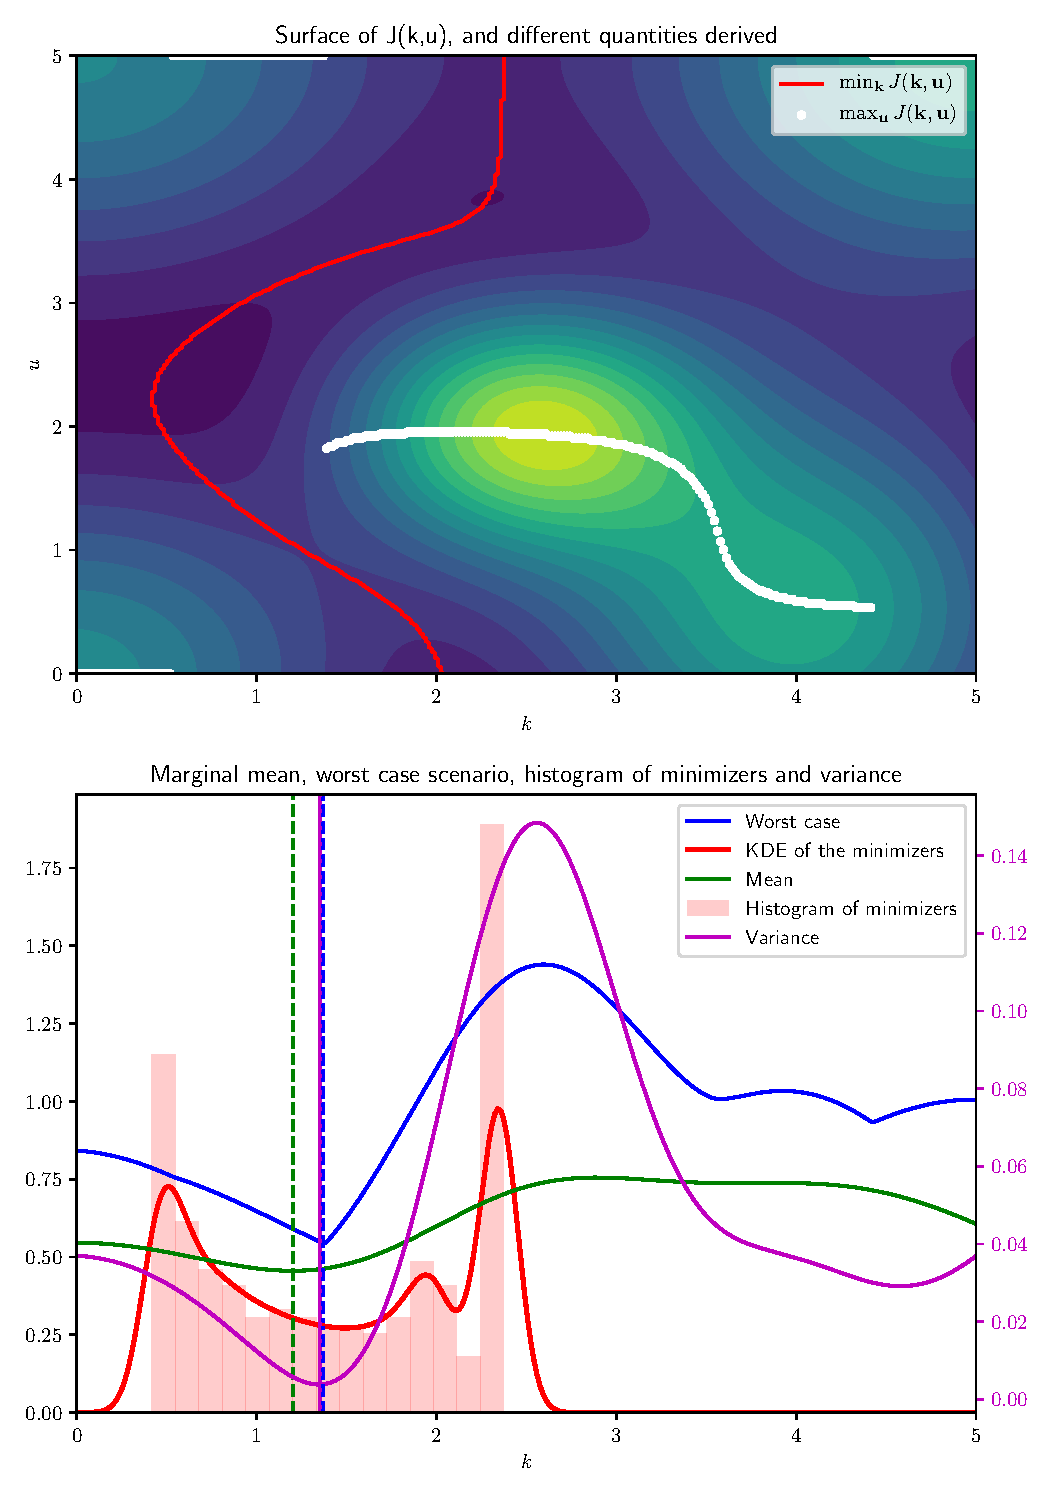
\includegraphics[scale=0.3]{summary_criteria}
                  %   \end{center}
                  %   % \pause
                  %   % Idea: Relaxation of the constraint:
                  %   % \begin{equation*}
                  %   %   R_{\alpha}(\bm{k}) = \Prob\left[J(\bm{k},\bm{U}) \leq \alpha \min_{\tilde{\bm{k}}} J(\tilde{\bm{k}},\bm{U})\right],\quad \alpha \geq 1
                  %   % \end{equation*}
                  %   % and increase $\alpha$ until $\max_{\bm{k}} R_{\alpha}(\bm{k})$ reaches a level of confidence.
                  % \end{column}
                % \end{columns}   %
              }
\begin{frame}
  \frametitle{Illustration}
  \pnote{
    What does it look like on a concrete example. We have the plot of a cost function, where k is the x axis, and u is on the y axis.

    As said earlier, for each horizontal cross section, so for a u fixed, we compute the minimiser, kstar of u.

    We can then compute the whole set of the conditional minimisers

    Now, we set alpha: inside the yellow lines, we are between the minimum and alpha times the minimum

    Finally, we construct and measure for each k the probability to be within this acceptable region.
   Great, now we just have to know how to choose alpha. Recalling that Gamma here is a probability, we can set levels of interests, such as 1, 0.9 or 0.95 for instance, and take the smallest alpha such that there is a value k where gamma of alpha and k reaches this level, similarly to a quantile.

  }
  \begin{columns}
    \begin{column}{0.4\textwidth}
  \includegraphics<1>[scale=0.35]{relaxation_tuto_1}
  \includegraphics<2>[scale=0.35]{relaxation_tuto_2}
  \includegraphics<3>[scale=0.35]{relaxation_tuto_3}
  \includegraphics<4->[scale=0.35]{relaxation_tuto_4}
\end{column}
\begin{column}{.6\textwidth}
  \begin{itemize}
  \item<1-> Sample $\bm{u}\sim\bm{U}$, and solve
   $\bm{k}^*(\bm{u}) = \argmin_{\bm{k}\in\Kspace} J(\bm{k},\bm{u})$
 \item<2->Set of conditional minimisers: $\{(\bm{k}^*(\bm{u}), \bm{u}) \mid \bm{u} \in \Uspace\}$
\item<3-> Set $\alpha \geq 1$
 \item<4-> $R_{\alpha}(\bm{k}) = \{\bm{u} \mid J(\bm{k},\bm{u}) < \alpha J^*(\bm{u}) \}$
 \item<4-> $\Gamma_{\alpha}(\bm{k}) = \Prob_{\bm{U}}\left[\bm{U}\in R_{\alpha}(\bm{k}) \right]$
   \item<5-> How to choose $\alpha$? When $\max_{\bm{k}} \Gamma_\alpha(\bm{k})$ reaches fixed levels
 \end{itemize}
\end{column}
  \end{columns}
\end{frame}

% \frame{
% \frametitle{Illustration of the relaxation}
% \begin{center}
% \scalebox{0.45}{%
% %% Creator: Matplotlib, PGF backend
%%
%% To include the figure in your LaTeX document, write
%%   \input{<filename>.pgf}
%%
%% Make sure the required packages are loaded in your preamble
%%   \usepackage{pgf}
%%
%% Figures using additional raster images can only be included by \input if
%% they are in the same directory as the main LaTeX file. For loading figures
%% from other directories you can use the `import` package
%%   \usepackage{import}
%% and then include the figures with
%%   \import{<path to file>}{<filename>.pgf}
%%
%% Matplotlib used the following preamble
%%   \usepackage{fontspec}
%%   \setmainfont{DejaVu Serif}
%%   \setsansfont{DejaVu Sans}
%%   \setmonofont{DejaVu Sans Mono}
%%
\begingroup%
\makeatletter%
\begin{pgfpicture}%
\pgfpathrectangle{\pgfpointorigin}{\pgfqpoint{9.340000in}{6.020000in}}%
\pgfusepath{use as bounding box, clip}%
\begin{pgfscope}%
\pgfsetbuttcap%
\pgfsetmiterjoin%
\definecolor{currentfill}{rgb}{1.000000,1.000000,1.000000}%
\pgfsetfillcolor{currentfill}%
\pgfsetlinewidth{0.000000pt}%
\definecolor{currentstroke}{rgb}{1.000000,1.000000,1.000000}%
\pgfsetstrokecolor{currentstroke}%
\pgfsetdash{}{0pt}%
\pgfpathmoveto{\pgfqpoint{0.000000in}{0.000000in}}%
\pgfpathlineto{\pgfqpoint{9.340000in}{0.000000in}}%
\pgfpathlineto{\pgfqpoint{9.340000in}{6.020000in}}%
\pgfpathlineto{\pgfqpoint{0.000000in}{6.020000in}}%
\pgfpathclose%
\pgfusepath{fill}%
\end{pgfscope}%
\begin{pgfscope}%
\pgfsetbuttcap%
\pgfsetmiterjoin%
\definecolor{currentfill}{rgb}{1.000000,1.000000,1.000000}%
\pgfsetfillcolor{currentfill}%
\pgfsetlinewidth{0.000000pt}%
\definecolor{currentstroke}{rgb}{0.000000,0.000000,0.000000}%
\pgfsetstrokecolor{currentstroke}%
\pgfsetstrokeopacity{0.000000}%
\pgfsetdash{}{0pt}%
\pgfpathmoveto{\pgfqpoint{0.848113in}{0.730900in}}%
\pgfpathlineto{\pgfqpoint{9.011271in}{0.730900in}}%
\pgfpathlineto{\pgfqpoint{9.011271in}{5.526350in}}%
\pgfpathlineto{\pgfqpoint{0.848113in}{5.526350in}}%
\pgfpathclose%
\pgfusepath{fill}%
\end{pgfscope}%
\begin{pgfscope}%
\pgfpathrectangle{\pgfqpoint{0.848113in}{0.730900in}}{\pgfqpoint{8.163158in}{4.795450in}}%
\pgfusepath{clip}%
\pgfsetbuttcap%
\pgfsetmiterjoin%
\definecolor{currentfill}{rgb}{0.000000,0.000000,1.000000}%
\pgfsetfillcolor{currentfill}%
\pgfsetfillopacity{0.100000}%
\pgfsetlinewidth{1.003750pt}%
\definecolor{currentstroke}{rgb}{0.000000,0.000000,1.000000}%
\pgfsetstrokecolor{currentstroke}%
\pgfsetstrokeopacity{0.100000}%
\pgfsetdash{}{0pt}%
\pgfpathmoveto{\pgfqpoint{1.376659in}{0.730900in}}%
\pgfpathlineto{\pgfqpoint{1.376659in}{5.526350in}}%
\pgfpathlineto{\pgfqpoint{1.704830in}{5.526350in}}%
\pgfpathlineto{\pgfqpoint{1.704830in}{0.730900in}}%
\pgfpathclose%
\pgfusepath{stroke,fill}%
\end{pgfscope}%
\begin{pgfscope}%
\pgfpathrectangle{\pgfqpoint{0.848113in}{0.730900in}}{\pgfqpoint{8.163158in}{4.795450in}}%
\pgfusepath{clip}%
\pgfsetbuttcap%
\pgfsetmiterjoin%
\definecolor{currentfill}{rgb}{0.000000,0.500000,0.000000}%
\pgfsetfillcolor{currentfill}%
\pgfsetfillopacity{0.100000}%
\pgfsetlinewidth{1.003750pt}%
\definecolor{currentstroke}{rgb}{0.000000,0.500000,0.000000}%
\pgfsetstrokecolor{currentstroke}%
\pgfsetstrokeopacity{0.100000}%
\pgfsetdash{}{0pt}%
\pgfpathmoveto{\pgfqpoint{2.024050in}{0.730900in}}%
\pgfpathlineto{\pgfqpoint{2.024050in}{5.526350in}}%
\pgfpathlineto{\pgfqpoint{6.103755in}{5.526350in}}%
\pgfpathlineto{\pgfqpoint{6.103755in}{0.730900in}}%
\pgfpathclose%
\pgfusepath{stroke,fill}%
\end{pgfscope}%
\begin{pgfscope}%
\pgfpathrectangle{\pgfqpoint{0.848113in}{0.730900in}}{\pgfqpoint{8.163158in}{4.795450in}}%
\pgfusepath{clip}%
\pgfsetbuttcap%
\pgfsetmiterjoin%
\definecolor{currentfill}{rgb}{1.000000,0.000000,0.000000}%
\pgfsetfillcolor{currentfill}%
\pgfsetfillopacity{0.100000}%
\pgfsetlinewidth{1.003750pt}%
\definecolor{currentstroke}{rgb}{1.000000,0.000000,0.000000}%
\pgfsetstrokecolor{currentstroke}%
\pgfsetstrokeopacity{0.100000}%
\pgfsetdash{}{0pt}%
\pgfpathmoveto{\pgfqpoint{5.351249in}{0.730900in}}%
\pgfpathlineto{\pgfqpoint{5.351249in}{5.526350in}}%
\pgfpathlineto{\pgfqpoint{7.723924in}{5.526350in}}%
\pgfpathlineto{\pgfqpoint{7.723924in}{0.730900in}}%
\pgfpathclose%
\pgfusepath{stroke,fill}%
\end{pgfscope}%
\begin{pgfscope}%
\pgfsetbuttcap%
\pgfsetroundjoin%
\definecolor{currentfill}{rgb}{0.000000,0.000000,0.000000}%
\pgfsetfillcolor{currentfill}%
\pgfsetlinewidth{0.803000pt}%
\definecolor{currentstroke}{rgb}{0.000000,0.000000,0.000000}%
\pgfsetstrokecolor{currentstroke}%
\pgfsetdash{}{0pt}%
\pgfsys@defobject{currentmarker}{\pgfqpoint{0.000000in}{-0.048611in}}{\pgfqpoint{0.000000in}{0.000000in}}{%
\pgfpathmoveto{\pgfqpoint{0.000000in}{0.000000in}}%
\pgfpathlineto{\pgfqpoint{0.000000in}{-0.048611in}}%
\pgfusepath{stroke,fill}%
}%
\begin{pgfscope}%
\pgfsys@transformshift{1.590218in}{0.730900in}%
\pgfsys@useobject{currentmarker}{}%
\end{pgfscope}%
\end{pgfscope}%
\begin{pgfscope}%
\pgftext[x=1.590218in,y=0.633678in,,top]{\sffamily\fontsize{10.000000}{12.000000}\selectfont \(\displaystyle 0\)}%
\end{pgfscope}%
\begin{pgfscope}%
\pgfsetbuttcap%
\pgfsetroundjoin%
\definecolor{currentfill}{rgb}{0.000000,0.000000,0.000000}%
\pgfsetfillcolor{currentfill}%
\pgfsetlinewidth{0.803000pt}%
\definecolor{currentstroke}{rgb}{0.000000,0.000000,0.000000}%
\pgfsetstrokecolor{currentstroke}%
\pgfsetdash{}{0pt}%
\pgfsys@defobject{currentmarker}{\pgfqpoint{0.000000in}{-0.048611in}}{\pgfqpoint{0.000000in}{0.000000in}}{%
\pgfpathmoveto{\pgfqpoint{0.000000in}{0.000000in}}%
\pgfpathlineto{\pgfqpoint{0.000000in}{-0.048611in}}%
\pgfusepath{stroke,fill}%
}%
\begin{pgfscope}%
\pgfsys@transformshift{3.074429in}{0.730900in}%
\pgfsys@useobject{currentmarker}{}%
\end{pgfscope}%
\end{pgfscope}%
\begin{pgfscope}%
\pgftext[x=3.074429in,y=0.633678in,,top]{\sffamily\fontsize{10.000000}{12.000000}\selectfont \(\displaystyle 1\)}%
\end{pgfscope}%
\begin{pgfscope}%
\pgfsetbuttcap%
\pgfsetroundjoin%
\definecolor{currentfill}{rgb}{0.000000,0.000000,0.000000}%
\pgfsetfillcolor{currentfill}%
\pgfsetlinewidth{0.803000pt}%
\definecolor{currentstroke}{rgb}{0.000000,0.000000,0.000000}%
\pgfsetstrokecolor{currentstroke}%
\pgfsetdash{}{0pt}%
\pgfsys@defobject{currentmarker}{\pgfqpoint{0.000000in}{-0.048611in}}{\pgfqpoint{0.000000in}{0.000000in}}{%
\pgfpathmoveto{\pgfqpoint{0.000000in}{0.000000in}}%
\pgfpathlineto{\pgfqpoint{0.000000in}{-0.048611in}}%
\pgfusepath{stroke,fill}%
}%
\begin{pgfscope}%
\pgfsys@transformshift{4.558639in}{0.730900in}%
\pgfsys@useobject{currentmarker}{}%
\end{pgfscope}%
\end{pgfscope}%
\begin{pgfscope}%
\pgftext[x=4.558639in,y=0.633678in,,top]{\sffamily\fontsize{10.000000}{12.000000}\selectfont \(\displaystyle 2\)}%
\end{pgfscope}%
\begin{pgfscope}%
\pgfsetbuttcap%
\pgfsetroundjoin%
\definecolor{currentfill}{rgb}{0.000000,0.000000,0.000000}%
\pgfsetfillcolor{currentfill}%
\pgfsetlinewidth{0.803000pt}%
\definecolor{currentstroke}{rgb}{0.000000,0.000000,0.000000}%
\pgfsetstrokecolor{currentstroke}%
\pgfsetdash{}{0pt}%
\pgfsys@defobject{currentmarker}{\pgfqpoint{0.000000in}{-0.048611in}}{\pgfqpoint{0.000000in}{0.000000in}}{%
\pgfpathmoveto{\pgfqpoint{0.000000in}{0.000000in}}%
\pgfpathlineto{\pgfqpoint{0.000000in}{-0.048611in}}%
\pgfusepath{stroke,fill}%
}%
\begin{pgfscope}%
\pgfsys@transformshift{6.042850in}{0.730900in}%
\pgfsys@useobject{currentmarker}{}%
\end{pgfscope}%
\end{pgfscope}%
\begin{pgfscope}%
\pgftext[x=6.042850in,y=0.633678in,,top]{\sffamily\fontsize{10.000000}{12.000000}\selectfont \(\displaystyle 3\)}%
\end{pgfscope}%
\begin{pgfscope}%
\pgfsetbuttcap%
\pgfsetroundjoin%
\definecolor{currentfill}{rgb}{0.000000,0.000000,0.000000}%
\pgfsetfillcolor{currentfill}%
\pgfsetlinewidth{0.803000pt}%
\definecolor{currentstroke}{rgb}{0.000000,0.000000,0.000000}%
\pgfsetstrokecolor{currentstroke}%
\pgfsetdash{}{0pt}%
\pgfsys@defobject{currentmarker}{\pgfqpoint{0.000000in}{-0.048611in}}{\pgfqpoint{0.000000in}{0.000000in}}{%
\pgfpathmoveto{\pgfqpoint{0.000000in}{0.000000in}}%
\pgfpathlineto{\pgfqpoint{0.000000in}{-0.048611in}}%
\pgfusepath{stroke,fill}%
}%
\begin{pgfscope}%
\pgfsys@transformshift{7.527060in}{0.730900in}%
\pgfsys@useobject{currentmarker}{}%
\end{pgfscope}%
\end{pgfscope}%
\begin{pgfscope}%
\pgftext[x=7.527060in,y=0.633678in,,top]{\sffamily\fontsize{10.000000}{12.000000}\selectfont \(\displaystyle 4\)}%
\end{pgfscope}%
\begin{pgfscope}%
\pgfsetbuttcap%
\pgfsetroundjoin%
\definecolor{currentfill}{rgb}{0.000000,0.000000,0.000000}%
\pgfsetfillcolor{currentfill}%
\pgfsetlinewidth{0.803000pt}%
\definecolor{currentstroke}{rgb}{0.000000,0.000000,0.000000}%
\pgfsetstrokecolor{currentstroke}%
\pgfsetdash{}{0pt}%
\pgfsys@defobject{currentmarker}{\pgfqpoint{0.000000in}{-0.048611in}}{\pgfqpoint{0.000000in}{0.000000in}}{%
\pgfpathmoveto{\pgfqpoint{0.000000in}{0.000000in}}%
\pgfpathlineto{\pgfqpoint{0.000000in}{-0.048611in}}%
\pgfusepath{stroke,fill}%
}%
\begin{pgfscope}%
\pgfsys@transformshift{9.011271in}{0.730900in}%
\pgfsys@useobject{currentmarker}{}%
\end{pgfscope}%
\end{pgfscope}%
\begin{pgfscope}%
\pgftext[x=9.011271in,y=0.633678in,,top]{\sffamily\fontsize{10.000000}{12.000000}\selectfont \(\displaystyle 5\)}%
\end{pgfscope}%
\begin{pgfscope}%
\pgftext[x=4.929692in,y=0.443710in,,top]{\sffamily\fontsize{10.000000}{12.000000}\selectfont \(\displaystyle {k}\)}%
\end{pgfscope}%
\begin{pgfscope}%
\pgfsetbuttcap%
\pgfsetroundjoin%
\definecolor{currentfill}{rgb}{0.000000,0.000000,0.000000}%
\pgfsetfillcolor{currentfill}%
\pgfsetlinewidth{0.803000pt}%
\definecolor{currentstroke}{rgb}{0.000000,0.000000,0.000000}%
\pgfsetstrokecolor{currentstroke}%
\pgfsetdash{}{0pt}%
\pgfsys@defobject{currentmarker}{\pgfqpoint{-0.048611in}{0.000000in}}{\pgfqpoint{0.000000in}{0.000000in}}{%
\pgfpathmoveto{\pgfqpoint{0.000000in}{0.000000in}}%
\pgfpathlineto{\pgfqpoint{-0.048611in}{0.000000in}}%
\pgfusepath{stroke,fill}%
}%
\begin{pgfscope}%
\pgfsys@transformshift{0.848113in}{0.730900in}%
\pgfsys@useobject{currentmarker}{}%
\end{pgfscope}%
\end{pgfscope}%
\begin{pgfscope}%
\pgftext[x=0.681446in,y=0.678139in,left,base]{\sffamily\fontsize{10.000000}{12.000000}\selectfont \(\displaystyle 0\)}%
\end{pgfscope}%
\begin{pgfscope}%
\pgfsetbuttcap%
\pgfsetroundjoin%
\definecolor{currentfill}{rgb}{0.000000,0.000000,0.000000}%
\pgfsetfillcolor{currentfill}%
\pgfsetlinewidth{0.803000pt}%
\definecolor{currentstroke}{rgb}{0.000000,0.000000,0.000000}%
\pgfsetstrokecolor{currentstroke}%
\pgfsetdash{}{0pt}%
\pgfsys@defobject{currentmarker}{\pgfqpoint{-0.048611in}{0.000000in}}{\pgfqpoint{0.000000in}{0.000000in}}{%
\pgfpathmoveto{\pgfqpoint{0.000000in}{0.000000in}}%
\pgfpathlineto{\pgfqpoint{-0.048611in}{0.000000in}}%
\pgfusepath{stroke,fill}%
}%
\begin{pgfscope}%
\pgfsys@transformshift{0.848113in}{1.689990in}%
\pgfsys@useobject{currentmarker}{}%
\end{pgfscope}%
\end{pgfscope}%
\begin{pgfscope}%
\pgftext[x=0.681446in,y=1.637229in,left,base]{\sffamily\fontsize{10.000000}{12.000000}\selectfont \(\displaystyle 2\)}%
\end{pgfscope}%
\begin{pgfscope}%
\pgfsetbuttcap%
\pgfsetroundjoin%
\definecolor{currentfill}{rgb}{0.000000,0.000000,0.000000}%
\pgfsetfillcolor{currentfill}%
\pgfsetlinewidth{0.803000pt}%
\definecolor{currentstroke}{rgb}{0.000000,0.000000,0.000000}%
\pgfsetstrokecolor{currentstroke}%
\pgfsetdash{}{0pt}%
\pgfsys@defobject{currentmarker}{\pgfqpoint{-0.048611in}{0.000000in}}{\pgfqpoint{0.000000in}{0.000000in}}{%
\pgfpathmoveto{\pgfqpoint{0.000000in}{0.000000in}}%
\pgfpathlineto{\pgfqpoint{-0.048611in}{0.000000in}}%
\pgfusepath{stroke,fill}%
}%
\begin{pgfscope}%
\pgfsys@transformshift{0.848113in}{2.649080in}%
\pgfsys@useobject{currentmarker}{}%
\end{pgfscope}%
\end{pgfscope}%
\begin{pgfscope}%
\pgftext[x=0.681446in,y=2.596319in,left,base]{\sffamily\fontsize{10.000000}{12.000000}\selectfont \(\displaystyle 4\)}%
\end{pgfscope}%
\begin{pgfscope}%
\pgfsetbuttcap%
\pgfsetroundjoin%
\definecolor{currentfill}{rgb}{0.000000,0.000000,0.000000}%
\pgfsetfillcolor{currentfill}%
\pgfsetlinewidth{0.803000pt}%
\definecolor{currentstroke}{rgb}{0.000000,0.000000,0.000000}%
\pgfsetstrokecolor{currentstroke}%
\pgfsetdash{}{0pt}%
\pgfsys@defobject{currentmarker}{\pgfqpoint{-0.048611in}{0.000000in}}{\pgfqpoint{0.000000in}{0.000000in}}{%
\pgfpathmoveto{\pgfqpoint{0.000000in}{0.000000in}}%
\pgfpathlineto{\pgfqpoint{-0.048611in}{0.000000in}}%
\pgfusepath{stroke,fill}%
}%
\begin{pgfscope}%
\pgfsys@transformshift{0.848113in}{3.608170in}%
\pgfsys@useobject{currentmarker}{}%
\end{pgfscope}%
\end{pgfscope}%
\begin{pgfscope}%
\pgftext[x=0.681446in,y=3.555409in,left,base]{\sffamily\fontsize{10.000000}{12.000000}\selectfont \(\displaystyle 6\)}%
\end{pgfscope}%
\begin{pgfscope}%
\pgfsetbuttcap%
\pgfsetroundjoin%
\definecolor{currentfill}{rgb}{0.000000,0.000000,0.000000}%
\pgfsetfillcolor{currentfill}%
\pgfsetlinewidth{0.803000pt}%
\definecolor{currentstroke}{rgb}{0.000000,0.000000,0.000000}%
\pgfsetstrokecolor{currentstroke}%
\pgfsetdash{}{0pt}%
\pgfsys@defobject{currentmarker}{\pgfqpoint{-0.048611in}{0.000000in}}{\pgfqpoint{0.000000in}{0.000000in}}{%
\pgfpathmoveto{\pgfqpoint{0.000000in}{0.000000in}}%
\pgfpathlineto{\pgfqpoint{-0.048611in}{0.000000in}}%
\pgfusepath{stroke,fill}%
}%
\begin{pgfscope}%
\pgfsys@transformshift{0.848113in}{4.567260in}%
\pgfsys@useobject{currentmarker}{}%
\end{pgfscope}%
\end{pgfscope}%
\begin{pgfscope}%
\pgftext[x=0.681446in,y=4.514499in,left,base]{\sffamily\fontsize{10.000000}{12.000000}\selectfont \(\displaystyle 8\)}%
\end{pgfscope}%
\begin{pgfscope}%
\pgfsetbuttcap%
\pgfsetroundjoin%
\definecolor{currentfill}{rgb}{0.000000,0.000000,0.000000}%
\pgfsetfillcolor{currentfill}%
\pgfsetlinewidth{0.803000pt}%
\definecolor{currentstroke}{rgb}{0.000000,0.000000,0.000000}%
\pgfsetstrokecolor{currentstroke}%
\pgfsetdash{}{0pt}%
\pgfsys@defobject{currentmarker}{\pgfqpoint{-0.048611in}{0.000000in}}{\pgfqpoint{0.000000in}{0.000000in}}{%
\pgfpathmoveto{\pgfqpoint{0.000000in}{0.000000in}}%
\pgfpathlineto{\pgfqpoint{-0.048611in}{0.000000in}}%
\pgfusepath{stroke,fill}%
}%
\begin{pgfscope}%
\pgfsys@transformshift{0.848113in}{5.526350in}%
\pgfsys@useobject{currentmarker}{}%
\end{pgfscope}%
\end{pgfscope}%
\begin{pgfscope}%
\pgftext[x=0.612002in,y=5.473589in,left,base]{\sffamily\fontsize{10.000000}{12.000000}\selectfont \(\displaystyle 10\)}%
\end{pgfscope}%
\begin{pgfscope}%
\pgftext[x=0.556446in,y=3.128625in,,bottom,rotate=90.000000]{\sffamily\fontsize{10.000000}{12.000000}\selectfont \(\displaystyle J({k},{u}_i)\)}%
\end{pgfscope}%
\begin{pgfscope}%
\pgfpathrectangle{\pgfqpoint{0.848113in}{0.730900in}}{\pgfqpoint{8.163158in}{4.795450in}}%
\pgfusepath{clip}%
\pgfsetrectcap%
\pgfsetroundjoin%
\pgfsetlinewidth{1.505625pt}%
\definecolor{currentstroke}{rgb}{0.000000,0.000000,1.000000}%
\pgfsetstrokecolor{currentstroke}%
\pgfsetdash{}{0pt}%
\pgfpathmoveto{\pgfqpoint{1.023844in}{5.536350in}}%
\pgfpathlineto{\pgfqpoint{1.039960in}{5.264992in}}%
\pgfpathlineto{\pgfqpoint{1.069704in}{4.793056in}}%
\pgfpathlineto{\pgfqpoint{1.099447in}{4.350008in}}%
\pgfpathlineto{\pgfqpoint{1.129191in}{3.935848in}}%
\pgfpathlineto{\pgfqpoint{1.158935in}{3.550577in}}%
\pgfpathlineto{\pgfqpoint{1.188678in}{3.194194in}}%
\pgfpathlineto{\pgfqpoint{1.218422in}{2.866699in}}%
\pgfpathlineto{\pgfqpoint{1.248166in}{2.568092in}}%
\pgfpathlineto{\pgfqpoint{1.277910in}{2.298373in}}%
\pgfpathlineto{\pgfqpoint{1.307653in}{2.057542in}}%
\pgfpathlineto{\pgfqpoint{1.337397in}{1.845599in}}%
\pgfpathlineto{\pgfqpoint{1.367141in}{1.662545in}}%
\pgfpathlineto{\pgfqpoint{1.396884in}{1.508378in}}%
\pgfpathlineto{\pgfqpoint{1.426628in}{1.383100in}}%
\pgfpathlineto{\pgfqpoint{1.456372in}{1.286710in}}%
\pgfpathlineto{\pgfqpoint{1.486115in}{1.219208in}}%
\pgfpathlineto{\pgfqpoint{1.515859in}{1.180594in}}%
\pgfpathlineto{\pgfqpoint{1.545603in}{1.170869in}}%
\pgfpathlineto{\pgfqpoint{1.575347in}{1.190031in}}%
\pgfpathlineto{\pgfqpoint{1.605090in}{1.238082in}}%
\pgfpathlineto{\pgfqpoint{1.634834in}{1.315020in}}%
\pgfpathlineto{\pgfqpoint{1.664578in}{1.420847in}}%
\pgfpathlineto{\pgfqpoint{1.694321in}{1.555562in}}%
\pgfpathlineto{\pgfqpoint{1.724065in}{1.719166in}}%
\pgfpathlineto{\pgfqpoint{1.753809in}{1.911657in}}%
\pgfpathlineto{\pgfqpoint{1.783552in}{2.133036in}}%
\pgfpathlineto{\pgfqpoint{1.813296in}{2.383304in}}%
\pgfpathlineto{\pgfqpoint{1.843040in}{2.662459in}}%
\pgfpathlineto{\pgfqpoint{1.872784in}{2.970503in}}%
\pgfpathlineto{\pgfqpoint{1.902527in}{3.307435in}}%
\pgfpathlineto{\pgfqpoint{1.932271in}{3.673255in}}%
\pgfpathlineto{\pgfqpoint{1.962015in}{4.067964in}}%
\pgfpathlineto{\pgfqpoint{1.991758in}{4.491560in}}%
\pgfpathlineto{\pgfqpoint{2.021502in}{4.944044in}}%
\pgfpathlineto{\pgfqpoint{2.057712in}{5.536350in}}%
\pgfpathlineto{\pgfqpoint{2.057712in}{5.536350in}}%
\pgfusepath{stroke}%
\end{pgfscope}%
\begin{pgfscope}%
\pgfpathrectangle{\pgfqpoint{0.848113in}{0.730900in}}{\pgfqpoint{8.163158in}{4.795450in}}%
\pgfusepath{clip}%
\pgfsetrectcap%
\pgfsetroundjoin%
\pgfsetlinewidth{1.505625pt}%
\definecolor{currentstroke}{rgb}{1.000000,0.000000,0.000000}%
\pgfsetstrokecolor{currentstroke}%
\pgfsetdash{}{0pt}%
\pgfpathmoveto{\pgfqpoint{4.098177in}{5.536350in}}%
\pgfpathlineto{\pgfqpoint{4.163048in}{5.332319in}}%
\pgfpathlineto{\pgfqpoint{4.252279in}{5.060770in}}%
\pgfpathlineto{\pgfqpoint{4.341510in}{4.799622in}}%
\pgfpathlineto{\pgfqpoint{4.400998in}{4.631300in}}%
\pgfpathlineto{\pgfqpoint{4.460485in}{4.467601in}}%
\pgfpathlineto{\pgfqpoint{4.519973in}{4.308523in}}%
\pgfpathlineto{\pgfqpoint{4.579460in}{4.154068in}}%
\pgfpathlineto{\pgfqpoint{4.638947in}{4.004235in}}%
\pgfpathlineto{\pgfqpoint{4.698435in}{3.859024in}}%
\pgfpathlineto{\pgfqpoint{4.757922in}{3.718435in}}%
\pgfpathlineto{\pgfqpoint{4.817410in}{3.582468in}}%
\pgfpathlineto{\pgfqpoint{4.876897in}{3.451123in}}%
\pgfpathlineto{\pgfqpoint{4.936384in}{3.324401in}}%
\pgfpathlineto{\pgfqpoint{4.995872in}{3.202300in}}%
\pgfpathlineto{\pgfqpoint{5.055359in}{3.084822in}}%
\pgfpathlineto{\pgfqpoint{5.114847in}{2.971965in}}%
\pgfpathlineto{\pgfqpoint{5.174334in}{2.863731in}}%
\pgfpathlineto{\pgfqpoint{5.233821in}{2.760119in}}%
\pgfpathlineto{\pgfqpoint{5.293309in}{2.661129in}}%
\pgfpathlineto{\pgfqpoint{5.352796in}{2.566761in}}%
\pgfpathlineto{\pgfqpoint{5.412284in}{2.477015in}}%
\pgfpathlineto{\pgfqpoint{5.471771in}{2.391892in}}%
\pgfpathlineto{\pgfqpoint{5.531258in}{2.311390in}}%
\pgfpathlineto{\pgfqpoint{5.590746in}{2.235511in}}%
\pgfpathlineto{\pgfqpoint{5.650233in}{2.164253in}}%
\pgfpathlineto{\pgfqpoint{5.709720in}{2.097618in}}%
\pgfpathlineto{\pgfqpoint{5.769208in}{2.035605in}}%
\pgfpathlineto{\pgfqpoint{5.828695in}{1.978214in}}%
\pgfpathlineto{\pgfqpoint{5.888183in}{1.925445in}}%
\pgfpathlineto{\pgfqpoint{5.947670in}{1.877298in}}%
\pgfpathlineto{\pgfqpoint{6.007157in}{1.833773in}}%
\pgfpathlineto{\pgfqpoint{6.066645in}{1.794870in}}%
\pgfpathlineto{\pgfqpoint{6.126132in}{1.760590in}}%
\pgfpathlineto{\pgfqpoint{6.185620in}{1.730931in}}%
\pgfpathlineto{\pgfqpoint{6.245107in}{1.705895in}}%
\pgfpathlineto{\pgfqpoint{6.304594in}{1.685481in}}%
\pgfpathlineto{\pgfqpoint{6.334338in}{1.677007in}}%
\pgfpathlineto{\pgfqpoint{6.364082in}{1.669688in}}%
\pgfpathlineto{\pgfqpoint{6.393826in}{1.663526in}}%
\pgfpathlineto{\pgfqpoint{6.423569in}{1.658518in}}%
\pgfpathlineto{\pgfqpoint{6.453313in}{1.654666in}}%
\pgfpathlineto{\pgfqpoint{6.483057in}{1.651970in}}%
\pgfpathlineto{\pgfqpoint{6.512800in}{1.650430in}}%
\pgfpathlineto{\pgfqpoint{6.542544in}{1.650044in}}%
\pgfpathlineto{\pgfqpoint{6.572288in}{1.650815in}}%
\pgfpathlineto{\pgfqpoint{6.602031in}{1.652741in}}%
\pgfpathlineto{\pgfqpoint{6.631775in}{1.655822in}}%
\pgfpathlineto{\pgfqpoint{6.661519in}{1.660059in}}%
\pgfpathlineto{\pgfqpoint{6.691263in}{1.665451in}}%
\pgfpathlineto{\pgfqpoint{6.721006in}{1.671999in}}%
\pgfpathlineto{\pgfqpoint{6.750750in}{1.679703in}}%
\pgfpathlineto{\pgfqpoint{6.810237in}{1.698576in}}%
\pgfpathlineto{\pgfqpoint{6.869725in}{1.722072in}}%
\pgfpathlineto{\pgfqpoint{6.929212in}{1.750190in}}%
\pgfpathlineto{\pgfqpoint{6.988699in}{1.782930in}}%
\pgfpathlineto{\pgfqpoint{7.048187in}{1.820292in}}%
\pgfpathlineto{\pgfqpoint{7.107674in}{1.862276in}}%
\pgfpathlineto{\pgfqpoint{7.167162in}{1.908882in}}%
\pgfpathlineto{\pgfqpoint{7.226649in}{1.960110in}}%
\pgfpathlineto{\pgfqpoint{7.286136in}{2.015961in}}%
\pgfpathlineto{\pgfqpoint{7.345624in}{2.076433in}}%
\pgfpathlineto{\pgfqpoint{7.405111in}{2.141528in}}%
\pgfpathlineto{\pgfqpoint{7.464599in}{2.211245in}}%
\pgfpathlineto{\pgfqpoint{7.524086in}{2.285583in}}%
\pgfpathlineto{\pgfqpoint{7.583573in}{2.364544in}}%
\pgfpathlineto{\pgfqpoint{7.643061in}{2.448127in}}%
\pgfpathlineto{\pgfqpoint{7.702548in}{2.536332in}}%
\pgfpathlineto{\pgfqpoint{7.762036in}{2.629160in}}%
\pgfpathlineto{\pgfqpoint{7.821523in}{2.726609in}}%
\pgfpathlineto{\pgfqpoint{7.881010in}{2.828680in}}%
\pgfpathlineto{\pgfqpoint{7.940498in}{2.935374in}}%
\pgfpathlineto{\pgfqpoint{7.999985in}{3.046689in}}%
\pgfpathlineto{\pgfqpoint{8.059473in}{3.162627in}}%
\pgfpathlineto{\pgfqpoint{8.118960in}{3.283187in}}%
\pgfpathlineto{\pgfqpoint{8.178447in}{3.408369in}}%
\pgfpathlineto{\pgfqpoint{8.237935in}{3.538173in}}%
\pgfpathlineto{\pgfqpoint{8.297422in}{3.672599in}}%
\pgfpathlineto{\pgfqpoint{8.356910in}{3.811647in}}%
\pgfpathlineto{\pgfqpoint{8.416397in}{3.955318in}}%
\pgfpathlineto{\pgfqpoint{8.475884in}{4.103610in}}%
\pgfpathlineto{\pgfqpoint{8.535372in}{4.256525in}}%
\pgfpathlineto{\pgfqpoint{8.594859in}{4.414061in}}%
\pgfpathlineto{\pgfqpoint{8.654347in}{4.576220in}}%
\pgfpathlineto{\pgfqpoint{8.713834in}{4.743001in}}%
\pgfpathlineto{\pgfqpoint{8.773321in}{4.914404in}}%
\pgfpathlineto{\pgfqpoint{8.832809in}{5.090429in}}%
\pgfpathlineto{\pgfqpoint{8.922040in}{5.363133in}}%
\pgfpathlineto{\pgfqpoint{8.977000in}{5.536350in}}%
\pgfpathlineto{\pgfqpoint{8.977000in}{5.536350in}}%
\pgfusepath{stroke}%
\end{pgfscope}%
\begin{pgfscope}%
\pgfpathrectangle{\pgfqpoint{0.848113in}{0.730900in}}{\pgfqpoint{8.163158in}{4.795450in}}%
\pgfusepath{clip}%
\pgfsetrectcap%
\pgfsetroundjoin%
\pgfsetlinewidth{1.505625pt}%
\definecolor{currentstroke}{rgb}{0.000000,0.500000,0.000000}%
\pgfsetstrokecolor{currentstroke}%
\pgfsetdash{}{0pt}%
\pgfpathmoveto{\pgfqpoint{0.838113in}{3.109195in}}%
\pgfpathlineto{\pgfqpoint{0.920985in}{3.023000in}}%
\pgfpathlineto{\pgfqpoint{1.010216in}{2.932725in}}%
\pgfpathlineto{\pgfqpoint{1.099447in}{2.845049in}}%
\pgfpathlineto{\pgfqpoint{1.188678in}{2.759974in}}%
\pgfpathlineto{\pgfqpoint{1.277910in}{2.677498in}}%
\pgfpathlineto{\pgfqpoint{1.367141in}{2.597622in}}%
\pgfpathlineto{\pgfqpoint{1.456372in}{2.520347in}}%
\pgfpathlineto{\pgfqpoint{1.545603in}{2.445671in}}%
\pgfpathlineto{\pgfqpoint{1.634834in}{2.373595in}}%
\pgfpathlineto{\pgfqpoint{1.724065in}{2.304119in}}%
\pgfpathlineto{\pgfqpoint{1.813296in}{2.237243in}}%
\pgfpathlineto{\pgfqpoint{1.902527in}{2.172967in}}%
\pgfpathlineto{\pgfqpoint{1.991758in}{2.111291in}}%
\pgfpathlineto{\pgfqpoint{2.080989in}{2.052214in}}%
\pgfpathlineto{\pgfqpoint{2.170221in}{1.995738in}}%
\pgfpathlineto{\pgfqpoint{2.259452in}{1.941862in}}%
\pgfpathlineto{\pgfqpoint{2.348683in}{1.890585in}}%
\pgfpathlineto{\pgfqpoint{2.437914in}{1.841909in}}%
\pgfpathlineto{\pgfqpoint{2.527145in}{1.795832in}}%
\pgfpathlineto{\pgfqpoint{2.616376in}{1.752356in}}%
\pgfpathlineto{\pgfqpoint{2.705607in}{1.711479in}}%
\pgfpathlineto{\pgfqpoint{2.794838in}{1.673202in}}%
\pgfpathlineto{\pgfqpoint{2.884069in}{1.637525in}}%
\pgfpathlineto{\pgfqpoint{2.973300in}{1.604448in}}%
\pgfpathlineto{\pgfqpoint{3.062531in}{1.573971in}}%
\pgfpathlineto{\pgfqpoint{3.151763in}{1.546094in}}%
\pgfpathlineto{\pgfqpoint{3.240994in}{1.520817in}}%
\pgfpathlineto{\pgfqpoint{3.330225in}{1.498140in}}%
\pgfpathlineto{\pgfqpoint{3.419456in}{1.478063in}}%
\pgfpathlineto{\pgfqpoint{3.508687in}{1.460585in}}%
\pgfpathlineto{\pgfqpoint{3.597918in}{1.445708in}}%
\pgfpathlineto{\pgfqpoint{3.687149in}{1.433431in}}%
\pgfpathlineto{\pgfqpoint{3.776380in}{1.423753in}}%
\pgfpathlineto{\pgfqpoint{3.865611in}{1.416675in}}%
\pgfpathlineto{\pgfqpoint{3.954842in}{1.412198in}}%
\pgfpathlineto{\pgfqpoint{4.044073in}{1.410320in}}%
\pgfpathlineto{\pgfqpoint{4.133305in}{1.411042in}}%
\pgfpathlineto{\pgfqpoint{4.222536in}{1.414364in}}%
\pgfpathlineto{\pgfqpoint{4.311767in}{1.420286in}}%
\pgfpathlineto{\pgfqpoint{4.400998in}{1.428808in}}%
\pgfpathlineto{\pgfqpoint{4.490229in}{1.439930in}}%
\pgfpathlineto{\pgfqpoint{4.579460in}{1.453652in}}%
\pgfpathlineto{\pgfqpoint{4.668691in}{1.469974in}}%
\pgfpathlineto{\pgfqpoint{4.757922in}{1.488896in}}%
\pgfpathlineto{\pgfqpoint{4.847153in}{1.510417in}}%
\pgfpathlineto{\pgfqpoint{4.936384in}{1.534539in}}%
\pgfpathlineto{\pgfqpoint{5.025615in}{1.561261in}}%
\pgfpathlineto{\pgfqpoint{5.114847in}{1.590582in}}%
\pgfpathlineto{\pgfqpoint{5.204078in}{1.622503in}}%
\pgfpathlineto{\pgfqpoint{5.293309in}{1.657025in}}%
\pgfpathlineto{\pgfqpoint{5.382540in}{1.694146in}}%
\pgfpathlineto{\pgfqpoint{5.471771in}{1.733867in}}%
\pgfpathlineto{\pgfqpoint{5.561002in}{1.776188in}}%
\pgfpathlineto{\pgfqpoint{5.650233in}{1.821109in}}%
\pgfpathlineto{\pgfqpoint{5.739464in}{1.868630in}}%
\pgfpathlineto{\pgfqpoint{5.828695in}{1.918751in}}%
\pgfpathlineto{\pgfqpoint{5.917926in}{1.971472in}}%
\pgfpathlineto{\pgfqpoint{6.007157in}{2.026793in}}%
\pgfpathlineto{\pgfqpoint{6.096389in}{2.084714in}}%
\pgfpathlineto{\pgfqpoint{6.185620in}{2.145234in}}%
\pgfpathlineto{\pgfqpoint{6.274851in}{2.208355in}}%
\pgfpathlineto{\pgfqpoint{6.364082in}{2.274075in}}%
\pgfpathlineto{\pgfqpoint{6.453313in}{2.342396in}}%
\pgfpathlineto{\pgfqpoint{6.542544in}{2.413316in}}%
\pgfpathlineto{\pgfqpoint{6.631775in}{2.486836in}}%
\pgfpathlineto{\pgfqpoint{6.721006in}{2.562957in}}%
\pgfpathlineto{\pgfqpoint{6.810237in}{2.641677in}}%
\pgfpathlineto{\pgfqpoint{6.899468in}{2.722997in}}%
\pgfpathlineto{\pgfqpoint{6.988699in}{2.806917in}}%
\pgfpathlineto{\pgfqpoint{7.077931in}{2.893437in}}%
\pgfpathlineto{\pgfqpoint{7.167162in}{2.982557in}}%
\pgfpathlineto{\pgfqpoint{7.256393in}{3.074277in}}%
\pgfpathlineto{\pgfqpoint{7.345624in}{3.168596in}}%
\pgfpathlineto{\pgfqpoint{7.434855in}{3.265516in}}%
\pgfpathlineto{\pgfqpoint{7.524086in}{3.365036in}}%
\pgfpathlineto{\pgfqpoint{7.613317in}{3.467155in}}%
\pgfpathlineto{\pgfqpoint{7.702548in}{3.571875in}}%
\pgfpathlineto{\pgfqpoint{7.791779in}{3.679194in}}%
\pgfpathlineto{\pgfqpoint{7.910754in}{3.826331in}}%
\pgfpathlineto{\pgfqpoint{8.029729in}{3.978090in}}%
\pgfpathlineto{\pgfqpoint{8.148704in}{4.134471in}}%
\pgfpathlineto{\pgfqpoint{8.267678in}{4.295474in}}%
\pgfpathlineto{\pgfqpoint{8.386653in}{4.461100in}}%
\pgfpathlineto{\pgfqpoint{8.505628in}{4.631347in}}%
\pgfpathlineto{\pgfqpoint{8.624603in}{4.806217in}}%
\pgfpathlineto{\pgfqpoint{8.743578in}{4.985708in}}%
\pgfpathlineto{\pgfqpoint{8.862552in}{5.169822in}}%
\pgfpathlineto{\pgfqpoint{8.981527in}{5.358558in}}%
\pgfpathlineto{\pgfqpoint{9.011271in}{5.406464in}}%
\pgfpathlineto{\pgfqpoint{9.011271in}{5.406464in}}%
\pgfusepath{stroke}%
\end{pgfscope}%
\begin{pgfscope}%
\pgfpathrectangle{\pgfqpoint{0.848113in}{0.730900in}}{\pgfqpoint{8.163158in}{4.795450in}}%
\pgfusepath{clip}%
\pgfsetbuttcap%
\pgfsetroundjoin%
\definecolor{currentfill}{rgb}{0.000000,0.000000,1.000000}%
\pgfsetfillcolor{currentfill}%
\pgfsetlinewidth{1.003750pt}%
\definecolor{currentstroke}{rgb}{0.000000,0.000000,1.000000}%
\pgfsetstrokecolor{currentstroke}%
\pgfsetdash{}{0pt}%
\pgfsys@defobject{currentmarker}{\pgfqpoint{-0.041667in}{-0.041667in}}{\pgfqpoint{0.041667in}{0.041667in}}{%
\pgfpathmoveto{\pgfqpoint{0.000000in}{-0.041667in}}%
\pgfpathcurveto{\pgfqpoint{0.011050in}{-0.041667in}}{\pgfqpoint{0.021649in}{-0.037276in}}{\pgfqpoint{0.029463in}{-0.029463in}}%
\pgfpathcurveto{\pgfqpoint{0.037276in}{-0.021649in}}{\pgfqpoint{0.041667in}{-0.011050in}}{\pgfqpoint{0.041667in}{0.000000in}}%
\pgfpathcurveto{\pgfqpoint{0.041667in}{0.011050in}}{\pgfqpoint{0.037276in}{0.021649in}}{\pgfqpoint{0.029463in}{0.029463in}}%
\pgfpathcurveto{\pgfqpoint{0.021649in}{0.037276in}}{\pgfqpoint{0.011050in}{0.041667in}}{\pgfqpoint{0.000000in}{0.041667in}}%
\pgfpathcurveto{\pgfqpoint{-0.011050in}{0.041667in}}{\pgfqpoint{-0.021649in}{0.037276in}}{\pgfqpoint{-0.029463in}{0.029463in}}%
\pgfpathcurveto{\pgfqpoint{-0.037276in}{0.021649in}}{\pgfqpoint{-0.041667in}{0.011050in}}{\pgfqpoint{-0.041667in}{0.000000in}}%
\pgfpathcurveto{\pgfqpoint{-0.041667in}{-0.011050in}}{\pgfqpoint{-0.037276in}{-0.021649in}}{\pgfqpoint{-0.029463in}{-0.029463in}}%
\pgfpathcurveto{\pgfqpoint{-0.021649in}{-0.037276in}}{\pgfqpoint{-0.011050in}{-0.041667in}}{\pgfqpoint{0.000000in}{-0.041667in}}%
\pgfpathclose%
\pgfusepath{stroke,fill}%
}%
\begin{pgfscope}%
\pgfsys@transformshift{1.540745in}{1.170483in}%
\pgfsys@useobject{currentmarker}{}%
\end{pgfscope}%
\end{pgfscope}%
\begin{pgfscope}%
\pgfpathrectangle{\pgfqpoint{0.848113in}{0.730900in}}{\pgfqpoint{8.163158in}{4.795450in}}%
\pgfusepath{clip}%
\pgfsetbuttcap%
\pgfsetroundjoin%
\definecolor{currentfill}{rgb}{1.000000,0.000000,0.000000}%
\pgfsetfillcolor{currentfill}%
\pgfsetlinewidth{1.003750pt}%
\definecolor{currentstroke}{rgb}{1.000000,0.000000,0.000000}%
\pgfsetstrokecolor{currentstroke}%
\pgfsetdash{}{0pt}%
\pgfsys@defobject{currentmarker}{\pgfqpoint{-0.041667in}{-0.041667in}}{\pgfqpoint{0.041667in}{0.041667in}}{%
\pgfpathmoveto{\pgfqpoint{0.000000in}{-0.041667in}}%
\pgfpathcurveto{\pgfqpoint{0.011050in}{-0.041667in}}{\pgfqpoint{0.021649in}{-0.037276in}}{\pgfqpoint{0.029463in}{-0.029463in}}%
\pgfpathcurveto{\pgfqpoint{0.037276in}{-0.021649in}}{\pgfqpoint{0.041667in}{-0.011050in}}{\pgfqpoint{0.041667in}{0.000000in}}%
\pgfpathcurveto{\pgfqpoint{0.041667in}{0.011050in}}{\pgfqpoint{0.037276in}{0.021649in}}{\pgfqpoint{0.029463in}{0.029463in}}%
\pgfpathcurveto{\pgfqpoint{0.021649in}{0.037276in}}{\pgfqpoint{0.011050in}{0.041667in}}{\pgfqpoint{0.000000in}{0.041667in}}%
\pgfpathcurveto{\pgfqpoint{-0.011050in}{0.041667in}}{\pgfqpoint{-0.021649in}{0.037276in}}{\pgfqpoint{-0.029463in}{0.029463in}}%
\pgfpathcurveto{\pgfqpoint{-0.037276in}{0.021649in}}{\pgfqpoint{-0.041667in}{0.011050in}}{\pgfqpoint{-0.041667in}{0.000000in}}%
\pgfpathcurveto{\pgfqpoint{-0.041667in}{-0.011050in}}{\pgfqpoint{-0.037276in}{-0.021649in}}{\pgfqpoint{-0.029463in}{-0.029463in}}%
\pgfpathcurveto{\pgfqpoint{-0.021649in}{-0.037276in}}{\pgfqpoint{-0.011050in}{-0.041667in}}{\pgfqpoint{0.000000in}{-0.041667in}}%
\pgfpathclose%
\pgfusepath{stroke,fill}%
}%
\begin{pgfscope}%
\pgfsys@transformshift{6.537587in}{1.650028in}%
\pgfsys@useobject{currentmarker}{}%
\end{pgfscope}%
\end{pgfscope}%
\begin{pgfscope}%
\pgfpathrectangle{\pgfqpoint{0.848113in}{0.730900in}}{\pgfqpoint{8.163158in}{4.795450in}}%
\pgfusepath{clip}%
\pgfsetbuttcap%
\pgfsetroundjoin%
\definecolor{currentfill}{rgb}{0.000000,0.500000,0.000000}%
\pgfsetfillcolor{currentfill}%
\pgfsetlinewidth{1.003750pt}%
\definecolor{currentstroke}{rgb}{0.000000,0.500000,0.000000}%
\pgfsetstrokecolor{currentstroke}%
\pgfsetdash{}{0pt}%
\pgfsys@defobject{currentmarker}{\pgfqpoint{-0.041667in}{-0.041667in}}{\pgfqpoint{0.041667in}{0.041667in}}{%
\pgfpathmoveto{\pgfqpoint{0.000000in}{-0.041667in}}%
\pgfpathcurveto{\pgfqpoint{0.011050in}{-0.041667in}}{\pgfqpoint{0.021649in}{-0.037276in}}{\pgfqpoint{0.029463in}{-0.029463in}}%
\pgfpathcurveto{\pgfqpoint{0.037276in}{-0.021649in}}{\pgfqpoint{0.041667in}{-0.011050in}}{\pgfqpoint{0.041667in}{0.000000in}}%
\pgfpathcurveto{\pgfqpoint{0.041667in}{0.011050in}}{\pgfqpoint{0.037276in}{0.021649in}}{\pgfqpoint{0.029463in}{0.029463in}}%
\pgfpathcurveto{\pgfqpoint{0.021649in}{0.037276in}}{\pgfqpoint{0.011050in}{0.041667in}}{\pgfqpoint{0.000000in}{0.041667in}}%
\pgfpathcurveto{\pgfqpoint{-0.011050in}{0.041667in}}{\pgfqpoint{-0.021649in}{0.037276in}}{\pgfqpoint{-0.029463in}{0.029463in}}%
\pgfpathcurveto{\pgfqpoint{-0.037276in}{0.021649in}}{\pgfqpoint{-0.041667in}{0.011050in}}{\pgfqpoint{-0.041667in}{0.000000in}}%
\pgfpathcurveto{\pgfqpoint{-0.041667in}{-0.011050in}}{\pgfqpoint{-0.037276in}{-0.021649in}}{\pgfqpoint{-0.029463in}{-0.029463in}}%
\pgfpathcurveto{\pgfqpoint{-0.021649in}{-0.037276in}}{\pgfqpoint{-0.011050in}{-0.041667in}}{\pgfqpoint{0.000000in}{-0.041667in}}%
\pgfpathclose%
\pgfusepath{stroke,fill}%
}%
\begin{pgfscope}%
\pgfsys@transformshift{4.063903in}{1.410256in}%
\pgfsys@useobject{currentmarker}{}%
\end{pgfscope}%
\end{pgfscope}%
\begin{pgfscope}%
\pgfpathrectangle{\pgfqpoint{0.848113in}{0.730900in}}{\pgfqpoint{8.163158in}{4.795450in}}%
\pgfusepath{clip}%
\pgfsetbuttcap%
\pgfsetroundjoin%
\pgfsetlinewidth{1.505625pt}%
\definecolor{currentstroke}{rgb}{0.000000,0.000000,1.000000}%
\pgfsetstrokecolor{currentstroke}%
\pgfsetdash{{5.550000pt}{2.400000pt}}{0.000000pt}%
\pgfpathmoveto{\pgfqpoint{1.376659in}{1.610066in}}%
\pgfpathlineto{\pgfqpoint{1.704830in}{1.610066in}}%
\pgfusepath{stroke}%
\end{pgfscope}%
\begin{pgfscope}%
\pgfpathrectangle{\pgfqpoint{0.848113in}{0.730900in}}{\pgfqpoint{8.163158in}{4.795450in}}%
\pgfusepath{clip}%
\pgfsetbuttcap%
\pgfsetroundjoin%
\pgfsetlinewidth{1.505625pt}%
\definecolor{currentstroke}{rgb}{0.000000,0.500000,0.000000}%
\pgfsetstrokecolor{currentstroke}%
\pgfsetdash{{5.550000pt}{2.400000pt}}{0.000000pt}%
\pgfpathmoveto{\pgfqpoint{2.024050in}{2.089611in}}%
\pgfpathlineto{\pgfqpoint{6.103755in}{2.089611in}}%
\pgfusepath{stroke}%
\end{pgfscope}%
\begin{pgfscope}%
\pgfpathrectangle{\pgfqpoint{0.848113in}{0.730900in}}{\pgfqpoint{8.163158in}{4.795450in}}%
\pgfusepath{clip}%
\pgfsetbuttcap%
\pgfsetroundjoin%
\pgfsetlinewidth{1.505625pt}%
\definecolor{currentstroke}{rgb}{1.000000,0.000000,0.000000}%
\pgfsetstrokecolor{currentstroke}%
\pgfsetdash{{5.550000pt}{2.400000pt}}{0.000000pt}%
\pgfpathmoveto{\pgfqpoint{5.351249in}{2.569156in}}%
\pgfpathlineto{\pgfqpoint{7.723924in}{2.569156in}}%
\pgfusepath{stroke}%
\end{pgfscope}%
\begin{pgfscope}%
\pgfsetrectcap%
\pgfsetmiterjoin%
\pgfsetlinewidth{0.803000pt}%
\definecolor{currentstroke}{rgb}{0.000000,0.000000,0.000000}%
\pgfsetstrokecolor{currentstroke}%
\pgfsetdash{}{0pt}%
\pgfpathmoveto{\pgfqpoint{0.848113in}{0.730900in}}%
\pgfpathlineto{\pgfqpoint{0.848113in}{5.526350in}}%
\pgfusepath{stroke}%
\end{pgfscope}%
\begin{pgfscope}%
\pgfsetrectcap%
\pgfsetmiterjoin%
\pgfsetlinewidth{0.803000pt}%
\definecolor{currentstroke}{rgb}{0.000000,0.000000,0.000000}%
\pgfsetstrokecolor{currentstroke}%
\pgfsetdash{}{0pt}%
\pgfpathmoveto{\pgfqpoint{9.011271in}{0.730900in}}%
\pgfpathlineto{\pgfqpoint{9.011271in}{5.526350in}}%
\pgfusepath{stroke}%
\end{pgfscope}%
\begin{pgfscope}%
\pgfsetrectcap%
\pgfsetmiterjoin%
\pgfsetlinewidth{0.803000pt}%
\definecolor{currentstroke}{rgb}{0.000000,0.000000,0.000000}%
\pgfsetstrokecolor{currentstroke}%
\pgfsetdash{}{0pt}%
\pgfpathmoveto{\pgfqpoint{0.848113in}{0.730900in}}%
\pgfpathlineto{\pgfqpoint{9.011271in}{0.730900in}}%
\pgfusepath{stroke}%
\end{pgfscope}%
\begin{pgfscope}%
\pgfsetrectcap%
\pgfsetmiterjoin%
\pgfsetlinewidth{0.803000pt}%
\definecolor{currentstroke}{rgb}{0.000000,0.000000,0.000000}%
\pgfsetstrokecolor{currentstroke}%
\pgfsetdash{}{0pt}%
\pgfpathmoveto{\pgfqpoint{0.848113in}{5.526350in}}%
\pgfpathlineto{\pgfqpoint{9.011271in}{5.526350in}}%
\pgfusepath{stroke}%
\end{pgfscope}%
\begin{pgfscope}%
\definecolor{textcolor}{rgb}{0.000000,0.000000,1.000000}%
\pgfsetstrokecolor{textcolor}%
\pgfsetfillcolor{textcolor}%
\pgftext[x=1.590218in,y=0.970673in,left,base]{\color{textcolor}\sffamily\fontsize{15.000000}{18.000000}\selectfont \(\displaystyle J(k^*_1,u_1)\)}%
\end{pgfscope}%
\begin{pgfscope}%
\definecolor{textcolor}{rgb}{0.000000,0.500000,0.000000}%
\pgfsetstrokecolor{textcolor}%
\pgfsetfillcolor{textcolor}%
\pgftext[x=4.113376in,y=1.546127in,left,base]{\color{textcolor}\sffamily\fontsize{15.000000}{18.000000}\selectfont \(\displaystyle J(k^*_2,u_2)\)}%
\end{pgfscope}%
\begin{pgfscope}%
\definecolor{textcolor}{rgb}{1.000000,0.000000,0.000000}%
\pgfsetstrokecolor{textcolor}%
\pgfsetfillcolor{textcolor}%
\pgftext[x=6.042850in,y=1.210445in,left,base]{\color{textcolor}\sffamily\fontsize{15.000000}{18.000000}\selectfont \(\displaystyle J(k^*_3,u_3)\)}%
\end{pgfscope}%
\begin{pgfscope}%
\pgftext[x=4.929692in,y=5.609684in,,base]{\sffamily\fontsize{12.000000}{14.400000}\selectfont \(\displaystyle J({k},{u}_i)\) for different \(\displaystyle {u}_i\), and regions of \(\displaystyle \mathcal{K}\) where \(\displaystyle J({k},{u}_i)\leq \alpha \min_{\tilde{k}}J(\tilde{k},{u}_i)\)}%
\end{pgfscope}%
\end{pgfpicture}%
\makeatother%
\endgroup%
}
% \end{center}
% }

             
\begin{frame}
  \frametitle{Choosing a $\alpha$}
  \pnote{
    Here we have our problem, and we are increasing alpha. The black curve in the bottom plot is gamma alpha of k. By increasing alpha, we increase the probability of being acceptable, and stop when this probability is 1. This can be seen on the top plot, there is a k, always in the acceptable region.
    What is interesting is that we have two informations. The value k of the estimation, but also the level alpha, that is controlling in a sense the regret we have relative to the best attainable performance.
  }
  \begin{center}
    \includegraphics<1>[height=.9\textheight, width= \textwidth]{branin0}
    \includegraphics<2>[height=.9\textheight, width= \textwidth]{branin1}
    \includegraphics<3>[height=.9\textheight, width= \textwidth]{branin2}
    \includegraphics<4>[height=.9\textheight, width= \textwidth]{branin3}
    \end{center}
  \end{frame}
  
\begin{frame}
  \frametitle{Bottlenecks and problems arising}
  \begin{itemize}
  \item Computational Bottlenecks
    \begin{itemize}
     \item Computer model: \alert{expensive to run} $\rightarrow$
    exhaustive computations unfeasible
  \item $\dim \Kspace$, $\dim \Uspace$?: \alert{curse of dimensionality}
  \end{itemize}
\item Calibration context
  \begin{itemize}
  \item How to assess quality of predictions
  \end{itemize}
  \end{itemize}
\end{frame}

\section{Surrogates}
\subsection{\small{How to compute $\hat{\bm{k}}$ in a reasonable time?}}
\frame[t]{
  \pnote{We now have defined an estimator, but it is really computationally expensive to run}
\frametitle{Why surrogates?}
\begin{itemize}
\item Replace expensive model by a computationally cheap metamodel ($\sim$ plug-in approach)
\item Adapted sequential procedures e.g. EGO
\item Uncertainties upon $\bm{u}$ may be incorporated directly in the surrogate
\end{itemize}
\vfill
\begin{center}
	\only<1>{\scalebox{0.9}{
\tikzstyle{block} = [rectangle, draw, fill=blue!20, 
     text centered, minimum width=1cm]
\tikzstyle{block2} = [rectangle, draw, fill=green!20, 
     text centered, , minimum width=6cm]

\tikzstyle{LHS}=[rectangle, draw, text centered]

\begin{tikzpicture}[node distance=3cm]

\node [align = center] at (0,0) (input) {Control variable \\$K \in \mathcal{K}$};
\node [align = center] at (4,1.5) (envir) {Environmental variables \\$\bm{X}_e$ random};
\node[block] at (4,0)(code){Direct Simulation};
\node[align = center] at (7,0) (output) {$W(\bm{x}_e,K)$};
\node[align = center] at (9.2,0) (jfun) {$j(\bm{x}_e,K)$};
\draw[->] (input) -- (code);
\draw[->] (envir) -- (code);
\draw[->] (code) -- (output);
\draw[->] (output) --(jfun);



\end{tikzpicture}}}	
	\only<2>{\scalebox{0.9}{
\tikzstyle{block} = [rectangle, draw, fill=blue!20, 
     text centered, minimum width=1cm]
\tikzstyle{block2} = [rectangle, draw, fill=green!20, 
     text centered, , minimum width=6cm]

\tikzstyle{LHS}=[rectangle, draw, text centered]

\begin{tikzpicture}[node distance=3cm]

\node [align = center] at (0,0) (input) {Control variable \\$K \in \mathcal{K}$};
\node [align = center] at (4,1.5) (envir) {Environmental variables \\$\bm{X}_e$ random};
\node[block] at (4,0)(code){Computer Code};
\node[align = center] at (7,0) (output) {$W(\bm{x}_e,K)$};
\node[align = center] at (9.2,0) (jfun) {$\bar{j}(\bm{x}_e,K)$};
\draw[->] (input) -- (code);
\draw[->] (envir) -- (code);
\draw[->] (code) -- (output);
\draw[->] (output) --(jfun);
\node[block2] at (5,0) (surr) {Metamodel};
\draw[->] (input) -- (surr);


\end{tikzpicture}}}
\end{center}
\vfill
Two main forms considered in UQ:\@
\begin{itemize}
\item Kriging (Gaussian Process Regression)~\cite{matheron_traite_1962}
\item Polynomial Chaos Expansion~\cite{xiu_wiener--askey_2002,sudret_polynomial_2015}
\end{itemize}
}

\begin{frame}
  \frametitle{Estimation of $\bm{K}^*$, $J^*(\bm{U})$}

  Iterative procedures to estimate set of conditional minimum/minimisers~\cite{ginsbourger_bayesian_2014}
  \begin{center}
  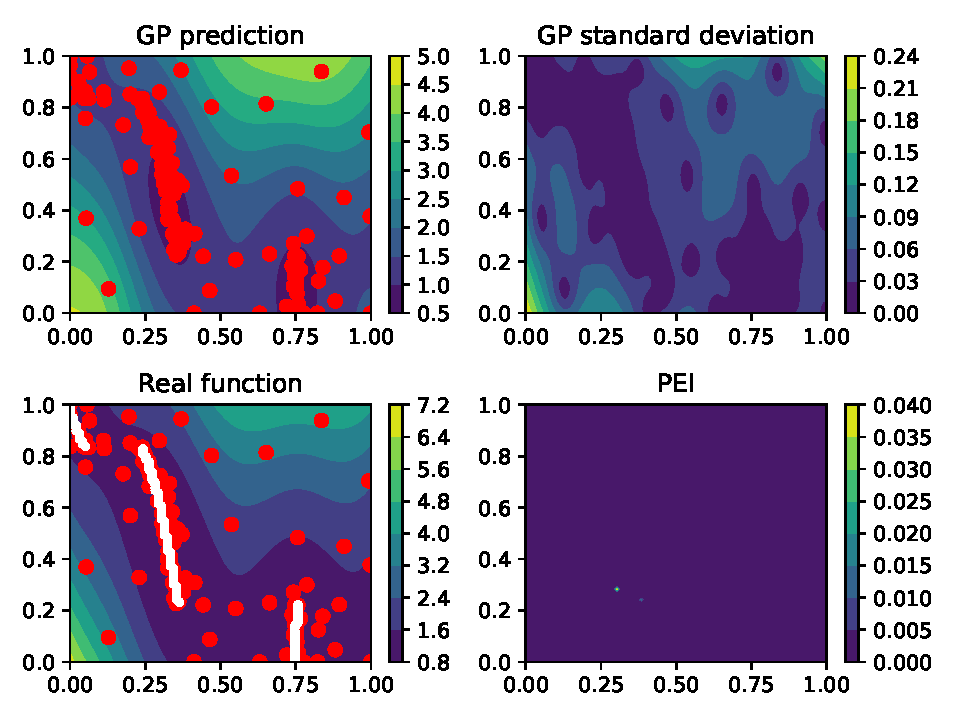
\includegraphics[scale=0.5]{PEI_branin}
\end{center}

\end{frame}

% \begin{frame}
%   \frametitle{Surrogates and dimension reduction}
%   \begin{itemize}
%   \item Sensitivity analysis~\cite{sudret_global_2008,le_gratiet_metamodel-based_2016}:
%     Based on intensive computation of the metamodel, or analytic computation based on coefficients of the expansion computed
%   \item Isotropic by groups kernels~\cite{blanchet-scalliet_specific_2017,ribaud_krigeage_2018-1}:
%     Group variables to have a few isotropic kernels
%   \end{itemize}

% \end{frame}

\metroset{sectionpage=progressbar, subsectionpage=none}

\section{Conclusion}
\frame{
\frametitle{Conclusion}
\begin{block}{Wrapping up}
\begin{itemize}
\item Problem of a \emph{good} definition of robustness
\item Strategies rely heavily on surrogate models, to embed aleatoric uncertainties directly in the modelling
\end{itemize}
\end{block}


\begin{block}{Perspective and future work}
\begin{itemize}
\item Cost of computer evaluations $\rightarrow$ limited number of runs?
\item Dimensionality of the input space $\rightarrow$ reduction of the input space?
\item How to deal with uncontrollable errors $\rightarrow$ realism of the model?
\end{itemize}
\end{block}
}
\begin{frame}[shrink=1
  ]
  \frametitle{References}
\bibliographystyle{alpha}
\bibliography{/home/victor/acadwriting/bibzotero.bib}
\end{frame}
\end{document}

%%% Local Variables:
%%% mode: latex
%%% TeX-master: t
%%% End:
